% The generic preamble
\documentclass[10pt,letterpaper,fleqn,titlepage]{report}

% Define packages to use
\usepackage{natbib}
\usepackage[dvips]{graphicx,color}
\usepackage{amsmath,amssymb}
\usepackage{bm}
\usepackage{caption}
\usepackage{xr}
\usepackage{ifthen}
\usepackage[dvipdfm,colorlinks,linkcolor=blue,citecolor=blue,urlcolor=blue]{hyperref}
\usepackage{fancybox}
\usepackage{textcomp}
\usepackage{fancyhdr}
\usepackage{titlesec}
\usepackage{multirow}
\usepackage{alltt}
\usepackage{svn}
\usepackage{longtable}

\titleformat{\chapter}[frame]
  {\normalfont}
  {\filright\slshape\Huge\enspace\thechapter\enspace}
  {8pt}
  {\normalfont\Huge\filcenter\slshape\sffamily} 

\titleformat{\section}[hang]
  {\normalfont}
  {\filright\sffamily\bfseries\Large\thesection}
  {5pt}
  {\normalfont\Large\filright\sffamily\bfseries}[\vspace{2pt}\titlerule]

\titleformat{\subsection}[hang]
  {\normalfont}
  {\filright\slshape\sffamily\large\thesubsection}
  {5pt}
  {\normalfont\large\filright\slshape\sffamily} 
  
% Redefine default page
\setlength{\textheight}{9.0in}  % 1" above and below
\setlength{\textwidth}{6.75in}   % 0.5" left and right
\setlength{\oddsidemargin}{-0.25in}
\setlength{\topmargin}{0.0pt}
\setlength{\headsep}{16.0pt}

% Redefine default paragraph
\setlength{\parindent}{0pt}
\setlength{\parskip}{1.5ex plus 0.5ex minus 0.2ex}

% Define caption width and default fonts
\setlength{\captionmargin}{0.5in}
\renewcommand{\captionfont}{\sffamily}
\renewcommand{\captionlabelfont}{\bfseries\sffamily}

% Defined commands
\newcommand{\superscript}[1]{\ensuremath{^\textrm{#1}}}
\newcommand{\subscript}[1]{\ensuremath{_\textrm{#1}}}
\newcommand{\invcm}{\textrm{cm\superscript{-1}}}
\newcommand{\micron}{\ensuremath{\mu\textrm{m}}}
\newcommand{\textbfm}[1]{\boldmath\ensuremath{#1}\unboldmath}
\newcommand{\water}{\textrm{H\subscript{2}O}}
\newcommand{\carbondioxide}{\textrm{CO\subscript{2}}}
\newcommand{\ozone}{\textrm{O\subscript{3}}}
\newcommand{\methane}{\textrm{CH\subscript{4}}}
\newcommand{\nitrousoxide}{\textrm{N\subscript{2}O}}
\newcommand{\carbonmonoxide}{\textrm{CO}}

% Define how equations are numbered
\numberwithin{equation}{chapter}
\numberwithin{figure}{chapter}
\numberwithin{table}{chapter}

% Space/nudging commands
\newcommand{\rb}[1]{\raisebox{1.5ex}[0pt]{#1}}

%Redefine the enumerate environment to decrease the item spacing.
\let\oldenumerate=\enumerate
\let\endoldenumerate=\endenumerate
\renewenvironment{enumerate}{%
  \begin{oldenumerate}%
    \setlength{\itemsep}{0ex}%
  }%
  {%
  \end{oldenumerate}%
  }

% Define a command for title page author email footnote
\newcommand{\email}[1]
{%
  \renewcommand{\thefootnote}{\alph{footnote}}%
  \footnote{#1}
  \renewcommand{\thefootnote}{\arabic{footnote}}
}

% Redefine the maketitle macro
\makeatletter
\renewcommand{\maketitle}
{%
  \thispagestyle{empty}
  \vspace*{1in}
  \begin{center}%
     \sffamily
     {\huge\bfseries Joint Center for Satellite Data Assimilation\par}%
  \end{center}
  \begin{flushleft}%
     \sffamily
     \vspace*{0.5in}
     {\Large\bfseries CRTM: \@title\par}%
     \medskip
     {\large\@author\par}%
     \medskip
     {\large\@date\par}%
     \bigskip\hrule\vspace*{2pc}%
  \end{flushleft}%
  \newpage
  \setcounter{footnote}{0}
}
\makeatother


% Define a command for a DRAFT watermark
\usepackage{eso-pic}
\newcommand{\draftwatermark}
{
  \AddToShipoutPicture{%
    \definecolor{lightgray}{gray}{.85}
    \setlength{\unitlength}{1in}
    \put(2.5,3.5){%
      \rotatebox{45}{%
        \resizebox{4in}{1in}{%
          \textsf{\textcolor{lightgray}{DRAFT}}
        }
      }
    }
  }
}


% Define included documents
\includeonly{Introduction,Get,Build,Use,StructDef.appendix,SensorId.appendix}

% Define fixed font for the various component names
\newcommand{\Atmosphere}{\texttt{Atmosphere}}
\newcommand{\Cloud}{\texttt{Cloud}}
\newcommand{\Aerosol}{\texttt{Aerosol}}
\newcommand{\Surface}{\texttt{Surface}}
\newcommand{\GeometryInfo}{\texttt{GeometryInfo}}
\newcommand{\ChannelInfo}{\texttt{ChannelInfo}}
\newcommand{\Options}{\texttt{Options}}
\newcommand{\AtmOptics}{\texttt{AtmOptics}}
\newcommand{\SfcOptics}{\texttt{SfcOptics}}
\newcommand{\RTSolution}{\texttt{RTSolution}}
\newcommand{\AtmAbsorption}{\texttt{AtmAbsorption}}
\newcommand{\AtmScatter}{\texttt{AtmScatter}}
\newcommand{\CloudScatter}{\texttt{CloudScatter}}
\newcommand{\AerosolScatter}{\texttt{AerosolScatter}}
% Generic fixed font command for Fortran95 syntax
\newcommand{\f}[1]{\texttt{#1}}
% Define the adjoint operator with correct spacing
\newcommand{\dstar}{\ensuremath{\delta^{*}\!}}
% Space/nudging commands
\newcommand{\rb}[1]{\raisebox{1.5ex}[0pt]{#1}}

%Redefine the enumerate environment to decrease the item spacing.
\let\oldenumerate=\enumerate
\let\endoldenumerate=\endenumerate
\renewenvironment{enumerate}{%
  \begin{oldenumerate}%
    \setlength{\itemsep}{0ex}%
  }%
  {%
  \end{oldenumerate}%
  }


% Title info
\title{v1.1 User Guide}
\author{Paul van Delst\email{paul.vandelst@noaa.gov}\\JCSDA/EMC/SAIC}
\date{July, 2008}


%-------------------------------------------------------------------------------
%                            Ze document begins...
%-------------------------------------------------------------------------------
\begin{document}
\maketitle

\draftwatermark

% The tables of content
%======================
\setcounter{page}{1}
\pagenumbering{roman}
  \tableofcontents\newpage
  \listoffigures\newpage
  \listoftables\newpage
\pagenumbering{arabic}
\setcounter{page}{1}


% Include all the sections
%=========================
\section{Introduction}
%=====================
A central design principle of the components of the CRTM Tangent-linear (TL) and Adjoint (AD) models is that the Forward model is always called first. Thus, in principle, forward model calculations are always available for the various TL and AD components.

The REL-1.1 CRTM AtmScatter modules obtained the interpolated cloud and aerosol optical properties from the CloudCoeff and AerosolCoeff lookup tables (LUTs) as shown in figure \ref{fig:AtmScatter_Interpolation}. For the tangent-linear and adjoint models (figures \ref{fig:AtmScatter_Interpolation}(b) and (c)), the necessary interpolation parameters such as the bracketing indices and interpolating polynomials were always recomputed.
 
\begin{figure}[htp]
  \centering
  % The generic preamble
\documentclass[10pt,letterpaper,fleqn,titlepage]{report}

% Define packages to use
\usepackage{natbib}
\usepackage[dvips]{graphicx,color}
\usepackage{amsmath,amssymb}
\usepackage{bm}
\usepackage{caption}
\usepackage{xr}
\usepackage{ifthen}
\usepackage[dvipdfm,colorlinks,linkcolor=blue,citecolor=blue,urlcolor=blue]{hyperref}
\usepackage{fancybox}
\usepackage{textcomp}
\usepackage{fancyhdr}
\usepackage{titlesec}
\usepackage{multirow}
\usepackage{alltt}
\usepackage{svn}
\usepackage{longtable}

\titleformat{\chapter}[frame]
  {\normalfont}
  {\filright\slshape\Huge\enspace\thechapter\enspace}
  {8pt}
  {\normalfont\Huge\filcenter\slshape\sffamily} 

\titleformat{\section}[hang]
  {\normalfont}
  {\filright\sffamily\bfseries\Large\thesection}
  {5pt}
  {\normalfont\Large\filright\sffamily\bfseries}[\vspace{2pt}\titlerule]

\titleformat{\subsection}[hang]
  {\normalfont}
  {\filright\slshape\sffamily\large\thesubsection}
  {5pt}
  {\normalfont\large\filright\slshape\sffamily} 
  
% Redefine default page
\setlength{\textheight}{9.0in}  % 1" above and below
\setlength{\textwidth}{6.75in}   % 0.5" left and right
\setlength{\oddsidemargin}{-0.25in}
\setlength{\topmargin}{0.0pt}
\setlength{\headsep}{16.0pt}

% Redefine default paragraph
\setlength{\parindent}{0pt}
\setlength{\parskip}{1.5ex plus 0.5ex minus 0.2ex}

% Define caption width and default fonts
\setlength{\captionmargin}{0.5in}
\renewcommand{\captionfont}{\sffamily}
\renewcommand{\captionlabelfont}{\bfseries\sffamily}

% Defined commands
\newcommand{\superscript}[1]{\ensuremath{^\textrm{#1}}}
\newcommand{\subscript}[1]{\ensuremath{_\textrm{#1}}}
\newcommand{\invcm}{\textrm{cm\superscript{-1}}}
\newcommand{\micron}{\ensuremath{\mu\textrm{m}}}
\newcommand{\textbfm}[1]{\boldmath\ensuremath{#1}\unboldmath}
\newcommand{\water}{\textrm{H\subscript{2}O}}
\newcommand{\carbondioxide}{\textrm{CO\subscript{2}}}
\newcommand{\ozone}{\textrm{O\subscript{3}}}
\newcommand{\methane}{\textrm{CH\subscript{4}}}
\newcommand{\nitrousoxide}{\textrm{N\subscript{2}O}}
\newcommand{\carbonmonoxide}{\textrm{CO}}

% Define how equations are numbered
\numberwithin{equation}{chapter}
\numberwithin{figure}{chapter}
\numberwithin{table}{chapter}

% Space/nudging commands
\newcommand{\rb}[1]{\raisebox{1.5ex}[0pt]{#1}}

%Redefine the enumerate environment to decrease the item spacing.
\let\oldenumerate=\enumerate
\let\endoldenumerate=\endenumerate
\renewenvironment{enumerate}{%
  \begin{oldenumerate}%
    \setlength{\itemsep}{0ex}%
  }%
  {%
  \end{oldenumerate}%
  }

% Define a command for title page author email footnote
\newcommand{\email}[1]
{%
  \renewcommand{\thefootnote}{\alph{footnote}}%
  \footnote{#1}
  \renewcommand{\thefootnote}{\arabic{footnote}}
}

% Redefine the maketitle macro
\makeatletter
\renewcommand{\maketitle}
{%
  \thispagestyle{empty}
  \vspace*{1in}
  \begin{center}%
     \sffamily
     {\huge\bfseries Joint Center for Satellite Data Assimilation\par}%
  \end{center}
  \begin{flushleft}%
     \sffamily
     \vspace*{0.5in}
     {\Large\bfseries CRTM: \@title\par}%
     \medskip
     {\large\@author\par}%
     \medskip
     {\large\@date\par}%
     \bigskip\hrule\vspace*{2pc}%
  \end{flushleft}%
  \newpage
  \setcounter{footnote}{0}
}
\makeatother


% Define a command for a DRAFT watermark
\usepackage{eso-pic}
\newcommand{\draftwatermark}
{
  \AddToShipoutPicture{%
    \definecolor{lightgray}{gray}{.85}
    \setlength{\unitlength}{1in}
    \put(2.5,3.5){%
      \rotatebox{45}{%
        \resizebox{4in}{1in}{%
          \textsf{\textcolor{lightgray}{DRAFT}}
        }
      }
    }
  }
}


% Define included documents
\includeonly{Optical_Property_Dependencies.section,Test_Cloud_and_Aerosol_Profiles.section,Forward_Model_Impact.section,Forward_Tangent-Linear_Model_Tests.section,Tangent-Linear_Adjoint_Model_Tests.section}


% Definitions for tables
\newcommand{\rb}[1]{\raisebox{1.5ex}[0pt]{#1}}
\newcommand{\po}{\ensuremath{p_{0}}}
\newcommand{\bpo}{\boldmath\po\unboldmath}
\newcommand{\Dp}{\ensuremath{\Delta p}}
\newcommand{\bDp}{\boldmath\Dp\unboldmath}
\newcommand{\reff}{\ensuremath{R_{eff}}}
\newcommand{\breff}{\boldmath\reff\unboldmath}
\newcommand{\bhpa}{\textbf{(hPa)}}
\newcommand{\bmicron}{\boldmath\micron\unboldmath}

% Title info
\title{Impact of Optical Property Interpolation on Atmospheric Scattering Computations}
\author{Paul van Delst\email{paul.vandelst@noaa.gov}\\JCSDA/EMC/SAIC}
\date{April, 2008}
\docnumber{(unassigned)}
\docseries{CRTM}


%-------------------------------------------------------------------------------
%                            Ze document begins...
%-------------------------------------------------------------------------------
\begin{document}
\maketitle

%\draftwatermark

\begin{abstract}
The CRTM interpolates the optical properties of clouds and aerosols from look-up tables (LUTs) for use in the scattering radiative transfer. This document details the impact of three different interpolation methodologies on the forward, tangent-linear and adjoint components of the cloud and aerosol scattering computations. Linear, cubic, and averaged quadratic inteprolation schemes were tested with the latter having the property of piecewise continuity of derivatives across LUT hingepoints.

\textbf{Keywords}: CRTM, scattering, clouds, aerosols, interpolation, derivative continuity
\end{abstract}


\section{Interpolation Schemes}
%==============================
For all of the CRTM cloud and aerosol optical property look-up table (LUT) interpolations described in this document, four different interpolation schemes were tested:
 \begin{itemize}
   \item{``old'' linear interpolation}
   \item{new linear interpolation}
   \item{cubic interpolation}
   \item{averaged quadratic interpolation}
 \end{itemize}
The difference between the old and new linear (or 2-point) interpolation routines are only in the way the interpolating polynomials are computed; the old scheme computed the polynomials explicitly like so,
\begin{eqnarray*}
  p_{1}(x) & = & \frac{x-x_{2}}{x_{1}-x_{2}} \\
  p_{2}(x) & = & \frac{x-x_{1}}{x_{2}-x_{1}}
\end{eqnarray*}
whereas the new scheme used the more generic form for computing Lagrangian polynomials for any set of $n+1$ points,
\begin{equation}
  p_{j}(x) = \prod_{\scriptstyle k=1 \atop \scriptstyle k \ne j}^{n+1}\frac{x-x_{k}}{x_{j}-x_{k}}
  \label{eqn:lagrangian_poly}
\end{equation}
with $n=1$. For cubic (or 4-point) interpolation, the same code was used but with $n=3$. In all cases the actual interpolating polynomial is computed using
\begin{equation}
  P(x) = \sum_{j=1}^{n+1} p_{j}(x)\cdot y_{j}
  \label{eqn:interpolating_poly}
\end{equation}

The averaged quadratic scheme\cite{Purser_AvgQuad_Interpolation} uses a weighted average of two adjacent 3-point (i.e. $n=2$) interpolating polynomials to perform interpolation in the overlapping region,
\begin{equation}
  P(x) = W_{l}\sum_{j=1}^{n+1} p_{j}(x)\cdot y_{j} + W_{r}\sum_{j=2}^{n+2} p_{j}(x)\cdot y_{j}
  \label{eqn:avgquad_poly}
\end{equation}
with
\begin{eqnarray*}
  W_{l} & = & 1 - \frac{x-x_{2}}{x_{3}-x_{2}}\\
   & & \\
  W_{r} & = & 1 - W_{l}
\end{eqnarray*}
This scheme preserves the interpolating function derivative continuity, in a piecewise fashion, across an interpolation boundary (also referred to here as a hingepoint). For end-point interpolation, the averaging weights are set accordingly to $W_{l}=1,W_{r}=0$, or $W_{l}=0,W_{r}=1$.

Comparisons between the old and new linear interpolation tests were run as a ``sanity-check'' only; they agreed and are not shown here. All of the subsequent test comparisons are between the linear, cubic, and averaged quadratic runs. Where applicable, tests were carried out for NOAA-18 HIRS/4, AMSU-A, and MHS; GOES-11 imager;  DMSP-16 SSMIS; and IASI Band 1 (645-1210\invcm) although not all the results are shown here. 

% Include all the various sections
%=================================
\section{Optical Property Dependencies}
%======================================

\subsection{Cloud Optical Properties}
%------------------------------------
The cloud optical property look-up table (LUT) contains extinction coefficient ($k_{e}$), single scatter albedo ($w$), asymmetry factor ($g$), and phase function Legendre polynomial coefficient ($P_{i}$) data for six different cloud types. These optical properties vary with repect to physical quantities such as frequency ($f$), effective particle radius ($R_{eff}$), temperature ($T$), and density ($\rho$). The data ranges for these independent variables in the current CRTM cloud optical properties LUT is shown in table \ref{tab:CloudCoeff.Independent.ranges}

\begin{table}[htp]
  \centering
  \begin{tabular}{|c | c | c|}
    \hline
    \textbf{Independent variable} & \textbf{Range} & \textbf{Units} \\
    \hline\hline
    Microwave frequency & 1.4-190.31   & GHz \\
    Infrared frequency  & 102-2902     & \invcm \\
    Microwave $R_{eff}$ & 10-1000      & \micron \\
    Infrared $R_{eff}$  & 5-100        & \micron \\
    Temperature         & 263.16-300.0 & K \\
    Density             & 0.1-0.9      & kg/m\superscript{3} \\
    \hline
  \end{tabular}
  \caption{The range of the independent data in the CRTM cloud optical properties LUT}
  \label{tab:CloudCoeff.Independent.ranges}
\end{table}

\begin{table}[htp]
  \centering
  \begin{tabular}{| c | c |}
    \hline
    \textbf{Data type} & \textbf{Dependency} \\
    \hline\hline
    Microwave frequencies, liquid phase & $f$, $R_{eff}$, $T$\\
    Microwave frequencies, solid phase  & $f$, $R_{eff}$, $\rho$\\
    Infrared frequencies, liquid phase & $f$, $R_{eff}$\\
    Infrared frequencies, solid phase  & $f$, $R_{eff}$, $\rho$\\
    \hline
  \end{tabular}
  \caption{The dependencies for the different gross data types  in the CRTM cloud optical properties LUT}
  \label{tab:CloudCoeff.Dependent.ranges}
\end{table}

For infrared frequencies, the cloud properties are interpolated across frequencies and radii for given densities; for microwave frequencies, the cloud properties are interpolated across frequency, radii and temperature (for liquid water clouds only) for given densities. Thus, depending on the spectral region and cloud type, one-, two-, or three-dimensional LUT interpolation may be performed, as shown in table \ref{tab:cloud_opt_interp}

\begin{table}[htp]
  \centering
  \begin{tabular}{|c | c | c|}
    \hline
    \textbf{Cloud Type} & \textbf{Infrared} & \textbf{Microwave} \\
    \hline\hline
    Water      & 2-D ($f,R_{eff}$) for $\rho_{0}$ & 2-D ($f,T$) for $R_{eff,1}$ \\
    Ice        & 2-D ($f,R_{eff}$) for $\rho_{3}$ & 1-D ($f$) for $R_{eff,1},\rho_{3}$\\
    Rain       & 2-D ($f,R_{eff}$) for $\rho_{0}$ & 3-D ($f,R_{eff},T$) \\
    Snow       & 2-D ($f,R_{eff}$) for $\rho_{1}$ & 2-D ($f,R_{eff}$) for $\rho_{1}$ \\
    Graupel    & 2-D ($f,R_{eff}$) for $\rho_{2}$ & 2-D ($f,R_{eff}$) for $\rho_{2}$ \\
    Hail       & 2-D ($f,R_{eff}$) for $\rho_{3}$ & 2-D ($f,R_{eff}$) for $\rho_{3}$ \\
    \hline
  \end{tabular}
  \caption{The type and dependency of the interpolation performed on the cloud optical properties.}
  \label{tab:cloud_opt_interp}
\end{table}


\subsection{Aerosol Optical Properties}
%--------------------------------------
Similar to the cloud optical property LUT, the aerosol optical property LUT contains $k_{e}$, $w$, $g$, and $P_{i}$ data for eight different aerosol types. The data ranges for these independent variables in the current CRTM aerosol optical properties LUT is shown in table \ref{tab:AerosolCoeff.Independent.ranges}

\begin{table}[htp]
  \centering
  \begin{tabular}{| c | c | c | c |}
    \hline
    \textbf{Independent variable} & \multicolumn{2}{|c|}{\textbf{Range}} & \textbf{Units} \\
    \hline\hline
    Frequency      & \multicolumn{2}{|c|}{250-3125}          & \invcm \\
    \hline
                   & Dust               &   0.0098 - 7.9887  & \\
                   & Sea salt-SSAM      &  0.79790 - 3.7987  & \\
                   & Sea salt-SSCM      &   5.7235 - 28.0934 & \\
                   & Dry Organic carbon &   0.0872 - 0.2122  & \\
    \rb{$R_{eff}$} & Wet Organic carbon &   0.0872 - 0.2122  & \rb{\micron} \\
                   & Dry Black carbon   &    0.039 - 0.0738  & \\
                   & Wet Black carbon   &    0.039 - 0.0738  & \\
                   & Sulfate            &   0.2424 - 0.7929  & \\
    \hline
  \end{tabular}
  \caption{The range of the independent data in the CRTM aerosol optical properties LUT}
  \label{tab:AerosolCoeff.Independent.ranges}
\end{table}

The aerosol data is organised differently in that different radii data are used for the different aerosol types and, thus, two-dimensional interpolation as a function of frequency and effective radius is used for all the aerosol types.

\section{Test Cloud and Aerosol Profiles}
%========================================
Six atmospheric profiles were used corresponding to the standard climatological profiles: Tropical, Midlatitude Summer, Midlatitude Winter, Subarctic Summer, Subarctic Winter, and the U.S. Standard Atmosphere.

Cloud and aerosol profiles were artificially constructed with only cursory correspondence to the climatology - the goal was simply to create a dataset that sufficiently exercises the source code.  The profile shapes were built as a function of pressure, $p$, using Gaussian-like functions,
\begin{equation}
  x(p) = \sum_{i=1}^{N} X_{i}\exp \left[ -\ln 2 \left(2\cdot \frac{|p-p_{0,i}|}{\Delta p_{i}}\right)^n\right]
\end{equation}
where $x \equiv R_{eff}$, cloud water content, or aerosol concentration; $p_{o}$ = the peak value layer pressure; $\Delta p$ = the peak pressure fullwidth at half maximum; and $X$ is the profile maximum value at $p_{o}$. For the effective radius profile, $n$=2, and for the water content and concentration profiles, $n$=3. The values used in constructing the six cloud and aerosol profiles are shown in tables \ref{tab:Test.Profile.cloud_parameters} and  \ref{tab:Test.Profile.aerosol_parameters}. Plots of the cloud and aerosol profiles are shown in figures \ref{fig:Test.Profile1} to \ref{fig:Test.Profile6}
 
\begin{table}[htp]
  \centering
  \begin{tabular}{|c|c|c|c|c|c|}
  \hline
  & & & & \multicolumn{2}{|c|}{\textbf{\itshape X}} \\
  \cline{5-6}
  \rb{\textbf{Cloud}} & \rb{\textbf{Associated}}  & \rb{\bpo}  & \rb{\bDp}  & \breff                & \textbf{Water content}\\
  \rb{\textbf{Type}}  & \rb{\textbf{Climatology}} & \rb{\bhpa} & \rb{\bhpa} & \bfseries{(\bmicron)} & \textbf{(kg/m\superscript{2})}\\
  \hline\hline
  Water   & Tropical           & 700 & 100 &   20 & 5 \\\hline
  Ice     & Subarctic summer   & 325 & 200 &  500 & 2 \\\hline
  Rain    & U.S. Std. Atm.     & 800 & 400 & 1000 & 5 \\\hline
  Snow    & Midlatitude winter & 400 & 200 &  500 & 1 \\\hline
  Graupel & Subarctic winter   & 800 & 100 & 1000 & 3 \\\hline
  Hail    & Midlatitude summer & 800 & 200 & 2000 & 2 \\\hline
  \end{tabular}
  \caption{Parameters used to construct the test cloud profiles.}
  \label{tab:Test.Profile.cloud_parameters}
\end{table}

\begin{table}[htp]
  \centering
  \begin{tabular}{|c|c|c|c|c|c|}
  \hline
  & & & & \multicolumn{2}{|c|}{\textbf{\itshape X}} \\
  \cline{5-6}
  \rb{\textbf{Aerosol}} & \rb{\textbf{Associated}}  & \rb{\bpo}  & \rb{\bDp}  & \breff                & \textbf{Concentration}\\
  \rb{\textbf{Type}}    & \rb{\textbf{Climatology}} & \rb{\bhpa} & \rb{\bhpa} & \bfseries{(\bmicron)} & \textbf{(kg/m\superscript{2})}\\
  \hline\hline
  Dust                    & Tropical                &  750 & 200 &    2 & 2.0   \\\hline
  Sea salt (SSAM)         & Subarctic summer        &  900 & 400 &  1.5 & 1.0   \\\hline
                          &                         &  800 & 200 & 0.15 & 0.06  \\\cline{3-6}
  \rb{Dry organic carbon} & \rb{U.S. Std. Atm.}     &  250 & 100 & 0.09 & 0.03  \\\hline
                          &                         &  800 & 200 & 0.15 & 0.4   \\\cline{3-6}
  \rb{Wet organic carbon} & \rb{Midlatitude winter} &  250 & 150 & 0.09 & 0.2   \\\hline
  Sea salt (SSCM)         & Subarctic winter        & 1000 & 200 & 12.0 & 0.05  \\\hline
                          &                         &  875 & 150 & 0.7  & 0.125 \\\cline{3-6}
  Sulfate                 & Midlatitude summer      &  600 & 200 & 0.45 & 0.05  \\\cline{3-6}
                          &                         &  200 & 100 & 0.3  & 0.03  \\\hline
  \end{tabular}
  \caption{Parameters used to construct the test aerosol profiles.}
  \label{tab:Test.Profile.aerosol_parameters}
\end{table}

\begin{figure}[htp]
  \centering
  \includegraphics[scale=1.0]{graphics/Test.Profile1.eps}
  \caption{Cloud and Aerosol data for Test Profile 1. Tropical climatology used for atmosphere.
    \textbf{(Upper panels)} Cloud profiles \textit{(a1)} Cloud water content \textit{(a2)} Cloud particle effective radius.
    \textbf{(Lower panels)} Aerosol profiles \textit{(b1)} Aerosol concentration \textit{(b2)} Aerosol particle effective radius.}
  \label{fig:Test.Profile1}
\end{figure}

\begin{figure}[htp]
  \centering
  \includegraphics[scale=1.0]{graphics/Test.Profile2.eps}
  \caption{Cloud and Aerosol data for Test Profile 2. Subarctic summer used for atmosphere.
    \textbf{(Upper panels)} Cloud profiles \textit{(a1)} Cloud water content \textit{(a2)} Cloud particle effective radius.
    \textbf{(Lower panels)} Aerosol profiles \textit{(b1)} Aerosol concentration \textit{(b2)} Aerosol particle effective radius.}
  \label{fig:Test.Profile2}
\end{figure}

\begin{figure}[htp]
  \centering
  \includegraphics[scale=1.0]{graphics/Test.Profile3.eps}
  \caption{Cloud and Aerosol data for Test Profile 3. U.S. Standard Atmosphere used for atmosphere.
    \textbf{(Upper panels)} Cloud profiles \textit{(a1)} Cloud water content \textit{(a2)} Cloud particle effective radius.
    \textbf{(Lower panels)} Aerosol profiles \textit{(b1)} Aerosol concentration \textit{(b2)} Aerosol particle effective radius.}
  \label{fig:Test.Profile3}
\end{figure}

\begin{figure}[htp]
  \centering
  \includegraphics[scale=1.0]{graphics/Test.Profile4.eps}
  \caption{Cloud and Aerosol data for Test Profile 4. Midlatitude winter used for atmosphere.
    \textbf{(Upper panels)} Cloud profiles \textit{(a1)} Cloud water content \textit{(a2)} Cloud particle effective radius.
    \textbf{(Lower panels)} Aerosol profiles \textit{(b1)} Aerosol concentration \textit{(b2)} Aerosol particle effective radius.}
  \label{fig:Test.Profile4}
\end{figure}

\begin{figure}[htp]
  \centering
  \includegraphics[scale=1.0]{graphics/Test.Profile5.eps}
  \caption{Cloud and Aerosol data for Test Profile 5. Subarctic winter used for atmosphere.
    \textbf{(Upper panels)} Cloud profiles \textit{(a1)} Cloud water content \textit{(a2)} Cloud particle effective radius.
    \textbf{(Lower panels)} Aerosol profiles \textit{(b1)} Aerosol concentration \textit{(b2)} Aerosol particle effective radius.}
  \label{fig:Test.Profile5}
\end{figure}

\begin{figure}[htp]
  \centering
  \includegraphics[scale=1.0]{graphics/Test.Profile6.eps}
  \caption{Cloud and Aerosol data for Test Profile 6. Midlatitude summer used for atmosphere.
    \textbf{(Upper panels)} Cloud profiles \textit{(a1)} Cloud water content \textit{(a2)} Cloud particle effective radius.
    \textbf{(Lower panels)} Aerosol profiles \textit{(b1)} Aerosol concentration \textit{(b2)} Aerosol particle effective radius.}
  \label{fig:Test.Profile6}
\end{figure}

\section{Forward Model Impact}
%=============================

\subsection{Clouds}
%------------------
The brightness temperature residuals that result from using different schemes for interpolation of the cloud optical properties for the test cloud profiles for NOAA-18 HIRS/4, NOAA-18 AMSU-A, and Band 1 of MetOp-A IASI are shown in figures \ref{fig:hirs4_n18.Differences.FWD.Cloud}, \ref{fig:amsua_n18.Differences.FWD.Cloud}, and \ref{fig:iasiB1_metop-a.Differences.FWD.Cloud} respectively.

Comparison of the clear-cloudy residuals to the interpolation residuals indicates that the latter is a small fraction of the former, but the magnitudes of the interpolation residuals can be relatively large, e.g. HIRS/4 and IASI hail and rain cloud cases, and AMSU-A ch.15 for most cloud cases. In addition, primarily for the infrared instruments, the differences between interpolation schemes alone can be relatively large which suggests that the residuals are overly influenced by anomalous interpolation due to low LUT data density. However, the interpretation of the interpolation residuals is somewhat complicated by the fact that the cloud optical properties used in the current CRTM version do not cover all the ranges of input data (e.g. effective radii, temperatures). This is discussed further in section  \ref{sec:Insufficient.LUT.range.Cloud}.
 
\begin{figure}[htp]
  \centering
  \textsf{\textbf{NOAA-18 HIRS/4}}\vspace{1.5ex}
  \includegraphics[bb=70 130 540 646,clip,scale=1.0]{graphics/Cloud/FWD/hirs4_n18.Differences.eps}
  \caption{Cloudy brightness temperature residuals for NOAA-18 HIRS/4. \textbf{(Left column)} Clear - Cloudy brightness temperature residuals. \textbf{(Centre column)} Cloudy calculation residuals due to difference in interpolated cloud optical properties from linear and cubic interpolation schemes. \textbf{(Right column)} Cloudy calculation residuals due to difference in interpolated cloud optical properties from linear and averaged quadratic interpolation schemes.}
  \label{fig:hirs4_n18.Differences.FWD.Cloud}
\end{figure}

\begin{figure}[htp]
  \centering
  \textsf{\textbf{NOAA-18 AMSU-A}}\vspace{1.5ex}
  \includegraphics[bb=70 130 540 646,clip,scale=1.0]{graphics/Cloud/FWD/amsua_n18.Differences.eps}
  \caption{Cloudy brightness temperature residuals for NOAA-18 AMSU-A. \textbf{(Left column)} Clear - Cloudy brightness temperature residuals. \textbf{(Centre column)} Cloudy calculation residuals due to difference in interpolated cloud optical properties from linear and cubic interpolation schemes. \textbf{(Right column)} Cloudy calculation residuals due to difference in interpolated cloud optical properties from linear and averaged quadratic interpolation schemes.}
  \label{fig:amsua_n18.Differences.FWD.Cloud}
\end{figure}

\begin{figure}[htp]
  \centering
  \textsf{\textbf{MetOp-A IASI (Band 1)}}\vspace{1.5ex}
  \includegraphics[bb=70 130 540 646,clip,scale=1.0]{graphics/Cloud/FWD/iasiB1_metop-a.Differences.eps}
  \caption{Cloudy brightness temperature residuals for MetOp-A IASI Band 1. \textbf{(Left column)} Clear - Cloudy brightness temperature residuals. \textbf{(Centre column)} Cloudy calculation residuals due to difference in interpolated cloud optical properties from linear and cubic  interpolation schemes. \textbf{(Right column)} Cloudy calculation residuals due to difference in interpolated cloud optical properties from linear and averaged quadratic interpolation schemes.}
  \label{fig:iasiB1_metop-a.Differences.FWD.Cloud}
\end{figure}

\subsection{Aerosols}
%--------------------
The brightness temperature residuals that result from different schemes for interpolation of the aerosol optical properties for the test aerosol profiles for NOAA-18 HIRS/4 and Band 1 of MetOp-A IASI are shown in figures \ref{fig:hirs4_n18.Differences.FWD.Aerosol} and \ref{fig:iasiB1_metop-a.Differences.FWD.Aerosol} respectively.

Compared to the cloudy interpolation residuals, the magnitudes of the same for aerosol optical properties is negligible. This could be a result of using a too-low aerosol burden in the test profiles. Alternatively, it could also indicate that the aerosol optical properties are either smoother in general with respect to the independent variables, or that they are simply more effectively represented in the LUT. The similarity between the residuals regardless of the interpolation scheme suggests the latter.

\begin{figure}[htp]
  \centering
  \textsf{\textbf{NOAA-18 HIRS/4}}\vspace{1.5ex}
  \includegraphics[bb=70 130 540 646,clip,scale=1.0]{graphics/Aerosol/FWD/hirs4_n18.Differences.eps}
  \caption{Aerosol brightness temperature residuals for NOAA-18 HIRS/4. \textbf{(Left column)} Clear - Aerosol brightness temperature residuals. \textbf{(Centre column)} Aerosol calculation residuals due to difference in interpolated aerosol optical properties from linear and cubic interpolation schemes. \textbf{(Right column)} Aerosol calculation residuals due to difference in interpolated aerosol optical properties from linear and averaged quadratic interpolation schemes.}
  \label{fig:hirs4_n18.Differences.FWD.Aerosol}
\end{figure}

\begin{figure}[htp]
  \centering
  \textsf{\textbf{MetOp-A IASI (Band 1)}}\vspace{1.5ex}
  \includegraphics[bb=70 130 540 646,clip,scale=1.0]{graphics/Aerosol/FWD/iasiB1_metop-a.Differences.eps}
  \caption{Aerosol brightness temperature residuals for MetOp-A IASI Band 1. \textbf{(Left column)} Clear - Aerosol brightness temperature residuals. \textbf{(Centre column)} Aerosol calculation residuals due to difference in interpolated aerosol optical properties from linear and cubic  interpolation schemes. \textbf{(Right column)} Aerosol calculation residuals due to difference in interpolated aerosol optical properties from linear and averaged quadratic interpolation schemes.}
  \label{fig:iasiB1_metop-a.Differences.FWD.Aerosol}
\end{figure}


\section{Forward/Tangent-Linear Model Tests}
%===========================================
Before discussing the results of the forward/tangent-linear model tests (FWD/TL test), a short description of the test itself is warranted. The FWD/TL test is not a ``pass-or-fail'' type of test, but is performed to allow assessment of the behaviour of the forward and tangent-linear model over a range of perturbations to the model variables. The input variables (temperature, cloud particle effective radius, and cloud water content for the CloudScatter test; aerosol particule effective radius and aerosol concentration for the AersosolScatter test) are perturbed 15 times decreasing from a maximum fraction of 0.1, with each subsequent perturbation being half of the previous one. Thus the final perturbation applied is approximately $6\times 10^{-6}$.
 
 
\subsection{CloudScatter Module}
%-------------------------------
\subsubsection{Insufficient range in LUT}
%........................................
\label{sec:Insufficient.LUT.range.Cloud}
Cases arise where the input cloud properties (temperature and effective radius) fall outside the range of data covered in the cloud optical properties LUT. In the forward model case, when this happens no extrapolation is performed - the LUT extrema values are simply returned. In the tangent-linear model case, the returned result is always zero.

A comparison of test output for the water cloud case for AMSU-A ch.8 (55.5GHz) inspecting the variation of the optical depth as a function of temperature is shown in figure \ref{fig:amsua_n18.ch8.WATER.dOd_dT}. The cloud optical property LUT temperature range is (currently) 263.16-300K. The layer cross-section shown in figure \ref{fig:amsua_n18.ch8.WATER.dOd_dT} is at 695hPa which, for the tropical climatology, has a temperature of 282.14K. The $\pm$0.1 perturbation fraction for the temperature yields 253.9K (-0.1) and 310.3K (+0.1). Because these values are outside the LUT temperature range, the forward model simply returns the 263.16 and 300K values for the -0.1 and +0.1 temperature perturbation respectively and that leads to the ``kinks'' in the non-linear response of figure \ref{fig:amsua_n18.ch8.WATER.dOd_dT}. Note that the feature occurs irrespective of the interpolation method. The tangent-linear result is not impacted in this particular case because the tangent-linear optical depth is not directly affected by the temperature perturbation, but only by the dependence of the mass extinction coefficient on the temperature perturbation - which, for temperatures outside the LUT range, is zero.

\begin{figure}[htp]
  \centering
  \begin{tabular}{c c c}
    \multicolumn{3}{c}{\qquad\sffamily\textbf{NOAA-18 AMSU-A ch.8}}\\
    \multicolumn{3}{c}{\qquad\sffamily\textbf{Water cloud test case}}\\
    \qquad\textsf{(a)} & \qquad\textsf{(b)}  & \qquad\textsf{(c)} \\
    \qquad\textsf{Linear} & \qquad\textsf{Cubic}  & \qquad\textsf{Averaged Quadratic} \\
    \includegraphics[bb=90 400 300 540,clip,scale=0.7]{graphics/Cloud/TL/amsua_n18.ch8.WATER.NLIN.dOd_dT.eps} &
    \includegraphics[bb=90 400 300 540,clip,scale=0.7]{graphics/Cloud/TL/amsua_n18.ch8.WATER.NCUBIC.dOd_dT.eps}  &
    \includegraphics[bb=90 400 300 540,clip,scale=0.7]{graphics/Cloud/TL/amsua_n18.ch8.WATER.AVGQUAD.dOd_dT.eps}
  \end{tabular}
  \caption{Effect of insufficient range in the cloud optical property LUT. Comparison of forward, non-linear (red) and tangent-linear (black) model optical depth variation with respect to temperature at 695hPa for the NOAA-18 AMSU-A ch.8 water cloud case using \textbf{(a)} linear, \textbf{(b)} cubic, and \textbf{(c)} averaged quadratic interpolation. The deviations in the non-linear response for the larger perturbations is due to the input cloud temperature data extending beyond that defined in the LUT. Symbol positions indicate the perturbation fractions at which the calculations were performed.}
  \label{fig:amsua_n18.ch8.WATER.dOd_dT}
\end{figure}

\subsubsection{Discontinuous Derivatives}
%........................................
\label{sec:Discontinuous.derivatives.Cloud}
The biggest problem for the simpler polynomial interpolation schemes being tested here is the fact that the interpolating function derivatives are discontinuous across LUT hingepoints. The effects of this appear as regular failures of linear interpolation and occasional failures of cubic interpolation. The following documents the character of this failures.

A comparison of test output for the snow cloud case for AMSU-A ch.8 (55.5GHz) inspecting the variation of the optical depth as a function of effective radius at 400hPa is shown in figure \ref{fig:amsua_n18.ch8.SNOW.dOd_dReff.TL}. Here, linear interpolation clearly highlights the derivative discontinuity when crossing over hinge-points in the LUT data. Inspection of the LUT dimension vectors lists the effective radii for the microwave cases as [10, 50, 250, 500, 750, 1000] and the test profile parameters for the snow cloud case shown in table \ref{tab:Test.Profile.cloud_parameters} indicate the maximum effective radius is 500\micron. Thus, as the forward model effective radius is perturbed beyond 500\micron, any subsequent linear interpolation of the LUT data will yield discontinuous derivatives. The linear case, figure \ref{fig:amsua_n18.ch8.SNOW.dOd_dReff.TL}(a), shows this most clearly: as soon as the effective radius changes from $<$500\micron{} to $>$500\micron, there is an abrupt change in the slope of the forward, non-linear result. This effect is not apparent in the corresponding plot for the cubic interpolation case but, as is shown later, that is due to a combination of the scale of the plot (i.e. the discontinuity is there, just not visible) and serendipity (i.e. it just so happens that the derivatives of the interpolating polynomials are nearly equal across the LUT hingepoint). The result using averaged quadratic interpolation, figure \ref{fig:amsua_n18.ch8.SNOW.dOd_dReff.TL}(c), appears similar to that for cubic interpolation, but with slightly different response curve slopes.

\begin{figure}[htp]
  \centering
  \begin{tabular}{c c c}
    \multicolumn{3}{c}{\qquad\sffamily\textbf{NOAA-18 AMSU-A ch.8}}\\
    \multicolumn{3}{c}{\qquad\sffamily\textbf{Snow cloud test case}}\\
    \qquad\textsf{(a)} & \qquad\textsf{(b)}  & \qquad\textsf{(c)} \\
    \qquad\textsf{Linear} & \qquad\textsf{Cubic}  & \qquad\textsf{Averaged Quadratic} \\
    \includegraphics[bb=90 400 300 540,clip,scale=0.7]{graphics/Cloud/TL/amsua_n18.ch8.SNOW.NLIN.dOd_dReff.eps} &
    \includegraphics[bb=90 400 300 540,clip,scale=0.7]{graphics/Cloud/TL/amsua_n18.ch8.SNOW.NCUBIC.dOd_dReff.eps} &
    \includegraphics[bb=90 400 300 540,clip,scale=0.7]{graphics/Cloud/TL/amsua_n18.ch8.SNOW.AVGQUAD.dOd_dReff.eps} 
  \end{tabular}
  \caption{Effect of discontinuous derivatives in the FWD/TL test. Comparison of forward, non-linear (red) and tangent-linear (black) model optical depth variation with respect to particle effective radius at 400hPa for the NOAA-18 AMSU-A ch.8 snow cloud case using different interpolation schemes. See figure \ref{fig:Test.Profile4} for the snow cloud water content and effective radius profiles.  \textbf{(a)} Linear interpolation. The abrubt change in the non-linear result slope occurs as the perturbations cross a LUT hingepoint (see text for details). \textbf{(b)} Cubic interpolation of the LUT data in this case does not lead to any noticable discontinuity. \textbf{(c)} Averaged quadratic interpolation preserves the derivatives across LUT higepoints, but note the slopes are slightly different. Symbol positions indicate the perturbation fractions at which the calculations were performed.}
  \label{fig:amsua_n18.ch8.SNOW.dOd_dReff.TL}
\end{figure}

A similar result is obtained in the snow cloud case for HIRS/4 ch.8 (900\invcm), but in this case the difference between cubic and averaged quadratic interpolation is more pronounced. Figure \ref{fig:hirs4_n18.ch8.SNOW.dg_dReff.TL} shows the variation of the asymmetry parameter with respect to effective radius at the 217hPa layer pressure (near the top of the snow cloud). For the linear interpolation case, we see the characteristic abrupt change in the non-linear slope across a LUT hinge-point, whereas for the cubic interpolation case the non-linear response is better behaved. The averaged quadratic interpolation result is quite different from the cubic interpolation case, with a significantly different tangent-linear slope, and a non-linear response that is more pronounced and with opposite curvature with respect to increasing perturbations.

\begin{figure}[htp]
  \centering
  \begin{tabular}{c c c}
    \multicolumn{3}{c}{\qquad\sffamily\textbf{NOAA-18 HIRS/4 ch.8}}\\
    \multicolumn{3}{c}{\qquad\sffamily\textbf{Snow cloud test case}}\\
    \qquad\textsf{(a)} & \qquad\textsf{(b)}  & \qquad\textsf{(c)} \\
    \qquad\textsf{Linear} & \qquad\textsf{Cubic}  & \qquad\textsf{Averaged Quadratic} \\
    \includegraphics[bb=90 400 300 540,clip,scale=0.7]{graphics/Cloud/TL/hirs4_n18.ch8.SNOW.NLIN.dg_dReff.eps} &
    \includegraphics[bb=90 400 300 540,clip,scale=0.7]{graphics/Cloud/TL/hirs4_n18.ch8.SNOW.NCUBIC.dg_dReff.eps} &
    \includegraphics[bb=90 400 300 540,clip,scale=0.7]{graphics/Cloud/TL/hirs4_n18.ch8.SNOW.AVGQUAD.dg_dReff.eps} 
  \end{tabular}
  \caption{Effect of discontinuous derivatives in the FWD/TL test. Comparison of forward, non-linear (red) and tangent-linear (black) model asymmetry parameter variation with respect to particle effective radius at 217hPa for the NOAA-18 HIRS/4 ch.8 snow cloud case using different interpolation schemes. See figure \ref{fig:Test.Profile4} for the snow cloud water content and effective radius profiles. \textbf{(a)} Linear interpolation. The abrubt change in the non-linear result slope occurs as the perturbations cross a LUT hingepoint (see text for details). \textbf{(b)} Cubic interpolation of the LUT data in this case does not lead to any noticeable discontinuity. \textbf{(c)} Averaged quadratic interpolation preserves the derivatives across LUT higepoints, but note the tangent-linear slope and character of the non-linar response are quite different from the cubic interpoaltion case. Symbol positions indicate the perturbation fractions at which the calculations were performed.}
  \label{fig:hirs4_n18.ch8.SNOW.dg_dReff.TL}
\end{figure}

A comparison of test results for the rain cloud case for AMSU-A ch.15 (89GHz), inspecting the variation of the optical depth as a function of effective radius at 918hPa, is shown in figure \ref{fig:amsua_n18.ch15.RAIN.dOd_dReff}. This case is mentioned because changing the interpolation scheme yields results that differ in sign: the linear interpolation scheme produces a negative tangent-linear slope, while the cubic and averaged quadratic produce a positive slope. Similarly for the non-linear response near zero perturbation.

\begin{figure}[htp]
  \centering
  \begin{tabular}{c c c}
    \multicolumn{3}{c}{\qquad\sffamily\textbf{NOAA-18 AMSU-A ch.15}}\\
    \multicolumn{3}{c}{\qquad\sffamily\textbf{Rain cloud test case}}\\
    \qquad\textsf{(a)} & \qquad\textsf{(b)}  & \qquad\textsf{(c)} \\
    \qquad\textsf{Linear} & \qquad\textsf{Cubic}  & \qquad\textsf{Averaged Quadratic} \\
    \includegraphics[bb=90 400 300 540,clip,scale=0.7]{graphics/Cloud/TL/amsua_n18.ch15.RAIN.NLIN.dOd_dReff.eps} &
    \includegraphics[bb=90 400 300 540,clip,scale=0.7]{graphics/Cloud/TL/amsua_n18.ch15.RAIN.NCUBIC.dOd_dReff.eps} &
    \includegraphics[bb=90 400 300 540,clip,scale=0.7]{graphics/Cloud/TL/amsua_n18.ch15.RAIN.AVGQUAD.dOd_dReff.eps} 
  \end{tabular}
  \caption{Impact of interpolation scheme on response slope. Comparison of forward, non-linear (red) and tangent-linear (black) model optical depth variation with respect to particle effective radius at 918hPa for the NOAA-18 AMSU-A ch.15 rain cloud case using different interpolation schemes. See figure \ref{fig:Test.Profile3} for the rain cloud water content and effective radius profiles. \textbf{(a)} Linear interpolation. Tangent-linear response, and non-linear response as $\delta x \rightarrow\pm 0$, have negative slope. \textbf{(b)} Cubic interpolation. Tangent-linear and non-linear response now have a positive slope. \textbf{(c)} Averaged quadratic interpolation produces a result similar to that using cubic interpolation but with a slightly different slope.
Symbol positions indicate the perturbation fractions at which the calculations were performed.}
  \label{fig:amsua_n18.ch15.RAIN.dOd_dReff}
\end{figure}

All of the previous FWD/TL test output has indicated that while linear interpolation produces spurious results in general, cubic interpolation works relatively well. However, there are many cases where simple polynomial interpolation does not produce good results, regardless of the order. Figure \ref{fig:hirs4_n18.ch8.WATER.dg_dReff.TL} shows the FWD/TL asymmetry parameter perturbation profiles due to effective radius perturbations for NOAA-18 HIRS/4 channel 8 water cloud test case at 695hPa. As the effective radius increases beyond a hinge-point, the linear interpolation case (figure \ref{fig:hirs4_n18.ch8.WATER.dg_dReff.TL}(a)) shows the characteristic abrubt change in the non-linear response. However, it also occurs for the cubic interpolation case (figure \ref{fig:hirs4_n18.ch8.WATER.dg_dReff.TL}(b)). Because the averaged quadratic interpolation scheme preserves derivative values across LUT hingepoint, the non-linear response is well-behaved about the hinge-point. Note also that the slope in the averaged quadratic case has the same sign as the linear case, and opposite to the cubic case. 

\begin{figure}[htp]
  \centering
  \begin{tabular}{c c c}
    \multicolumn{3}{c}{\qquad\sffamily\textbf{NOAA-18 HIRS/4 ch.8}}\\
    \multicolumn{3}{c}{\qquad\sffamily\textbf{Water cloud test case}}\\
    \qquad\textsf{(a)} & \qquad\textsf{(b)}  & \qquad\textsf{(c)} \\
    \qquad\textsf{Linear} & \qquad\textsf{Cubic}  & \qquad\textsf{Averaged Quadratic} \\
    \includegraphics[bb=90 400 300 540,clip,scale=0.7]{graphics/Cloud/TL/hirs4_n18.ch8.WATER.NLIN.dg_dReff.eps} &
    \includegraphics[bb=90 400 300 540,clip,scale=0.7]{graphics/Cloud/TL/hirs4_n18.ch8.WATER.NCUBIC.dg_dReff.eps} &
    \includegraphics[bb=90 400 300 540,clip,scale=0.7]{graphics/Cloud/TL/hirs4_n18.ch8.WATER.AVGQUAD.dg_dReff.eps} 
  \end{tabular}
  \caption{Demonstration that cubic interpolation also suffers from the discontinuous derivative problem. Comparison of forward, non-linear (red) and tangent-linear (black) model asymmetry parameter variation with respect to particle effective radius for the NOAA-18 HIRS/4 ch.8 water cloud case using different interpolation schemes. See figure \ref{fig:Test.Profile1} for the water cloud water content and effective radius profiles. \textbf{(a)} Linear interpolation. The abrubt change in the non-linear result slope occurs as the perturbations cross a LUT hingepoint. \textbf{(b)} Cubic interpolation also exhibits the abrupt change in the non-linear response across a LUT hingepoint. \textbf{(c)} Averaged quadratic interpolation preserves derivatives across LUT hingepoints so the non-linear response is well-behaved. Note the change in the sign of the response curve slopes for the different interpolation schemes. Symbol positions indicate the perturbation fractions at which the calculations were performed.}
  \label{fig:hirs4_n18.ch8.WATER.dg_dReff.TL}
\end{figure}

Closer inspection of the actual LUT data indicates why the cubic interpolation scheme performs so poorly with respect to the non-linear response in this case: the data are distributed in such a fashion as to produce large discontinuities in the derivatives across an interpolation higepoint. Figure \ref{fig:g_IR.Reff.898cm-1}(a) shows the water cloud asymmetry parameter LUT data plotted as a function of effective radius for 898\invcm{} (approximately the central frequency of HIRS channel 8) with the cubic and averaged quadratic interpolates superimposed. For the perturbation shown in figure \ref{fig:hirs4_n18.ch8.WATER.dg_dReff.TL}, the effective radius varies from about 18 to 22\micron, with the zero perturbation value for the selected pressure layer being around 18.5\micron. Returning to figure \ref{fig:g_IR.Reff.898cm-1}(a), as the effective radius passes the hinge-point at 20\micron{} (labeled point \#3), the cubic interpolation switches from the red curve to the green curve, which have very different slopes close to the 20\micron{} hingepoint, leading to the corresponding change in the non-linear response seen in figure \ref{fig:hirs4_n18.ch8.WATER.dg_dReff.TL}. For averaged quadratic interpolation, crossing the 20\micron{} hingepoint changes the interpolation from the cyan to the magenta curve which by definition have the same slope at the hingepoint. This is clearly shown in figure \ref{fig:g_IR.Reff.898cm-1}(b) where the derivative of the cubic polynomial interpolates are clearly very different at 20\micron{}, whereas those for the averaged quadratic interpolates are piecewise continuous.

\begin{figure}[htp]
  \centering
  \includegraphics[scale=0.8]{graphics/Cloud/g_IR.Reff.898cm-1.eps}
  \caption{Comparison of interpolation schemes across a cloud optical properties LUT hingepoint. \textbf{(a)} The asymmetry factor is interpolated as a function of effective radius for a single infrared frequency, 898\invcm. The interpolation is being performed in the specified range of effective radii about the 20\micron{} radius hingepoint. \textbf{(b)} The derivatives of the cubic and averaged quadratic interpolation schemes shown in (a). The derivatives of the adjacent cubic polynomials are very different (i.e. discontinuous) at the LUT hingepoint ($R_{eff}=20$\micron), whereas those for the averaged quadratic interpolation are piecewise continuous.}
  \label{fig:g_IR.Reff.898cm-1}
\end{figure}

A series of tests were performed to see if transforming the variables that are interpolated would make a different in this particular case. Both the dependent and independent variables were transformed individually and together. The dependent variable transforms\cite{Purser_Variable_Transform} used were,

\parbox{10cm}{\begin{eqnarray*}
                y & = & \frac{2g-1}{\sqrt{1-(2g-1)^{2}}}\\
                g & = & \frac{1}{2}+\frac{y}{2\sqrt{1+y^{2}}}
              \end{eqnarray*}}\hfill
\parbox{1cm}{\begin{eqnarray}\end{eqnarray}}

and the independent variable transform\cite{Purser_Variable_Transform} used was simply,
\begin{equation}
  x = \frac{1}{r}
  \label{eqn:r_transform}
\end{equation}
Transforming just the asymmetry parameter before interpolating produced a result similar to that for no transformation except that the magnitude of the excursions in the points 1-4 higher order interpolations were slightly reduced from that of figure \ref{fig:g_IR.Reff.898cm-1}.

Transforming the independent variable prior to interpolation produced a slightly better result as seen in figure \ref{fig:g_IR.Reff.898cm-1.r_transformed}(a). The point 1-4 cubic interpolation curve provides a qualitatively better representation of the LUT data although the difference between it and the point 2-5 interpolation curve is still evident. The excursion now seen for the point 2-5 interpolation curve between points 2 and 3 is never used for interpolation, but its appearance does highlight the potential for poor interpolates due to low LUT data density. The interpolate derivatives, shown in figure \ref{fig:g_IR.Reff.898cm-1.r_transformed}(b), behave similarly to the untransformed case.

\begin{figure}[htp]
  \centering
  \includegraphics[scale=0.8]{graphics/Cloud/g_IR.Reff.898cm-1.r_transformed.eps} \\
  \caption{Comparison of interpolation schemes across a cloud optical properties LUT hingepoint when the independent variable is transformed according to eqn.\ref{eqn:r_transform}. Compare with figure \ref{fig:g_IR.Reff.898cm-1}.}
  \label{fig:g_IR.Reff.898cm-1.r_transformed}
\end{figure}

Transforming both the dependent and independent variables prior to interpolation produced results similar to that for just the independent variable transform shown in figure \ref{fig:g_IR.Reff.898cm-1.r_transformed}(a) but with a larger excursion for the points 2-5 interpolation curve between points 2 and 3.

None of the results for the interpolations shown in figures \ref{fig:g_IR.Reff.898cm-1}(a) or \ref{fig:g_IR.Reff.898cm-1.r_transformed}(a) are particularly satisfactory. It is clear that better representation of the cloud optical properties is needed by increasing the LUT data density. 


\subsection{AerosolScatter Module}
%---------------------------------
\subsubsection{Insufficient range in LUT}
%........................................
\label{sec:Insufficient.LUT.range.Aerosol}
As with the CloudScatter tests described in section \ref{sec:Insufficient.LUT.range.Cloud}, the AerosolScatter LUT interpolation produces similar results when the input data lies outside the range of the LUT data. Figure \ref{fig:hirs4_n18.ch8.SSAM.dw_dReff} shows the impact of this effect for single scatter albedo as a function of effective radius for NOAA-18 HIRS/4 ch.8 for the sea salt (SSAM) aerosol test case. Comparison with figure \ref{fig:amsua_n18.ch8.WATER.dOd_dT} shows the same characteristic discontinuity.

\begin{figure}[htp]
  \centering
  \begin{tabular}{c c c}
    \multicolumn{3}{c}{\qquad\sffamily\textbf{NOAA-18 HIRS/4 ch.8}}\\
    \multicolumn{3}{c}{\qquad\sffamily\textbf{Sea Salt (SSAM) test case}}\\
    \qquad\textsf{(a)} & \qquad\textsf{(b)}  & \qquad\textsf{(c)} \\
    \qquad\textsf{Linear} & \qquad\textsf{Cubic}  & \qquad\textsf{Averaged Quadratic} \\
    \includegraphics[bb=90 400 300 540,clip,scale=0.7]{graphics/Aerosol/TL/hirs4_n18.ch8.SSAM.NLIN.dw_dReff.eps} &
    \includegraphics[bb=90 400 300 540,clip,scale=0.7]{graphics/Aerosol/TL/hirs4_n18.ch8.SSAM.NCUBIC.dw_dReff.eps} &
    \includegraphics[bb=90 400 300 540,clip,scale=0.7]{graphics/Aerosol/TL/hirs4_n18.ch8.SSAM.AVGQUAD.dw_dReff.eps} 
  \end{tabular}
  \caption{Effect of insufficient range in the aerosol optical property LUT. Comparison of forward, non-linear (red) and tangent-linear (black) model single scatter albedo variation with respect to effective radius at 718hPa for the NOAA-18 HIRS/4 ch.8 sea salt (SSAM) case using \textbf{(a)} linear, \textbf{(b)} cubic, and \textbf{(c)} averaged quadratic interpolation. The deviations in the non-linear response for the larger perturbations is due to the input aerosol effective radius data extending beyond that defined in the LUT. Symbol positions indicate the perturbation fractions at which the calculations were performed. See figure \ref{fig:Test.Profile2} for the sea salt (SSAM) aerosol concentration and effective radius profiles.}
  \label{fig:hirs4_n18.ch8.SSAM.dw_dReff}
\end{figure}


\subsubsection{Discontinous derivatives and discretised LUT data}
%................................................................
As with the CloudScatter tests described in section \ref{sec:Discontinuous.derivatives.Cloud}, the use of a simple polynomial interpolating function does not preserve the continuity of derivatives across LUT hingepoints. This effect is exacerbated in the aerosol optical property interpolation by discretisation of the data. Figure \ref{fig:hirs4_n18.ch8.SSCM.dg_dReff} shows the impact of this effect for the asymmetry factor as a function of effective radius for NOAA-18 HIRS/4 ch.8 for the sea salt (SSCM) aerosol test case. Note that the typical abrupt change is seen in the reponse plots, but the position where it occurs changes with the interpolation method used, and the non-linear response is quite poor in general for the entire range of perturbations; something that was not seen in the CloudScatter interpolations. For the CloudScatter case we saw the data in question was not represented at a high enough data density for interpolation to perform well; in this case, it appears the slight discretisation of the LUT data along the y-axis coupled with the irregular spacing in the x-axis is the cause of poor non-linear response for this case, as shown in figure \ref{fig:g.Reff.SSCM.900cm-1}. Figure \ref{fig:g.Reff.SSCM.900cm-1}(b) shows the significant difference between the interpolating functions either side of a LUT hingepoint (in this case $\sim$11.41\micron.)

\begin{figure}[htp]
  \centering
  \begin{tabular}{c c c}
    \multicolumn{3}{c}{\qquad\sffamily\textbf{NOAA-18 HIRS/4 ch.8}}\\
    \multicolumn{3}{c}{\qquad\sffamily\textbf{Sea Salt (SSCM) test case}}\\
    \qquad\textsf{(a)} & \qquad\textsf{(b)}  & \qquad\textsf{(c)} \\
    \qquad\textsf{Linear} & \qquad\textsf{Cubic}  & \qquad\textsf{Averaged Quadratic} \\
    \includegraphics[bb=90 400 300 540,clip,scale=0.7]{graphics/Aerosol/TL/hirs4_n18.ch8.SSCM.NLIN.dg_dReff.eps} &
    \includegraphics[bb=90 400 300 540,clip,scale=0.7]{graphics/Aerosol/TL/hirs4_n18.ch8.SSCM.NCUBIC.dg_dReff.eps} &
    \includegraphics[bb=90 400 300 540,clip,scale=0.7]{graphics/Aerosol/TL/hirs4_n18.ch8.SSCM.AVGQUAD.dg_dReff.eps} 
  \end{tabular}
  \caption{Effect of discretised data when interpolating LUT aerosol optical property data. Comparison of forward, non-linear (red) and tangent-linear (black) model asymmetry parameter variation with respect to effective radius at 972hPa for the NOAA-18 HIRS/4 ch.8 sea salt (SSAM) case using \textbf{(a)} linear, \textbf{(b)} cubic, and \textbf{(c)} averaged quadratic interpolation. Symbol positions indicate the perturbation fractions at which the calculations were performed. See figure \ref{fig:Test.Profile5} for the sea salt (SSCM) aerosol concentration and effective radius profiles.}
  \label{fig:hirs4_n18.ch8.SSCM.dg_dReff}
\end{figure}

\begin{figure}[htp]
  \centering
  \includegraphics[scale=0.8]{graphics/Aerosol/g.Reff.SSCM.900cm-1.eps}
  \caption{Comparison of interpolation across a aerosol optical property LUT hingepoint where the data is partially discretised. \textbf{(a)} The sea salt (SSCM) asymmetry factor as a function of effective radius for a single infrared frequency of 900\invcm. \textbf{(b)} Zoom of a portion of the plot in (a) showing the respective interpolation curves for interpolation being performed about the $\sim$11.4\micron{} radius hingepoint. The character of the cubic interpolating function generated using points 1-4 (red curve) is different from that generated using points 2-5 (green curve). The averaged quadratic interpolations are more well behaved about the LUT hingepoint.}
  \label{fig:g.Reff.SSCM.900cm-1}
\end{figure}

\section{Tangent-Linear/Adjoint Model Tests}
%===========================================
The tangent-linear/adjoint (TL/AD) test is a simpler one than the FWD/TL test. In this test both the CloudScatter and AerosolScatter tangent-linear and adjoint models are run with successive inputs given a value of 1.0. The subsequent TL output and transpose of the AD output should agree to within numerical precision. This should be true regardless of the LUT interpolation scheme used, and it was found to be so. The results shown here are simply an additional documentation of the difference between the adjoint model outputs that are due to the interpolation method.

\subsection{CloudScatter Module}
%-------------------------------
Using the snow cloud case for AMSU-A ch.8 again, the differences between the three interpolation methods  in the adjoint model is shown in figure \ref{fig:amsua_n18.ch8.SNOW.dOd_dReff.AD}. The Jacobian profile for the linear interpolation case, figure \ref{fig:amsua_n18.ch8.SNOW.dOd_dReff.AD}(a), is significantly different in shape and magnitude compared to either the cubic or averaged quadratic interpolation results. The differences between the cubic and averaged quadratic interpolation results are more subtle with the latter having a slightly larger peak value than the former.
\begin{figure}[htp]
  \centering
  \begin{tabular}{c c c}
    \multicolumn{3}{c}{\qquad\sffamily\textbf{NOAA-18 AMSU-A ch.8}}\\
    \multicolumn{3}{c}{\qquad\sffamily\textbf{Snow cloud test case}}\\
    \qquad\textsf{(a)} & \qquad\textsf{(b)}  & \qquad\textsf{(c)} \\
    \qquad\textsf{Linear} & \qquad\textsf{Cubic}  & \qquad\textsf{Averaged Quadratic} \\
    \includegraphics[bb=90 400 300 540,clip,scale=0.7]{graphics/Cloud/AD/amsua_n18.ch8.SNOW.NLIN.dOd_dReff.eps} &
    \includegraphics[bb=90 400 300 540,clip,scale=0.7]{graphics/Cloud/AD/amsua_n18.ch8.SNOW.NCUBIC.dOd_dReff.eps} &
    \includegraphics[bb=90 400 300 540,clip,scale=0.7]{graphics/Cloud/AD/amsua_n18.ch8.SNOW.AVGQUAD.dOd_dReff.eps} \\
  \end{tabular}
  \caption{Comparison of the tangent-linear (black) and adjoint (red) model optical depth variation with respect to effective radius profile for the NOAA-18 AMSU-A ch.8 snow cloud case using \textbf{(a)} linear, \textbf{(b)} cubic, and \textbf{(c)} averaged quadratic interpolation. See figure \ref{fig:Test.Profile4} for the snow cloud water content and effective radius profiles.}
  \label{fig:amsua_n18.ch8.SNOW.dOd_dReff.AD}
\end{figure}

A similar comparison for the rain cloud case for AMSU-A channel 15 is shown in figure \ref{fig:amsua_n18.ch15.RAIN.dw_dReff.AD}. In this example, the case of figure \ref{fig:amsua_n18.ch15.RAIN.dw_dReff.AD}(a) clearly shows the shortcomings of using linear interpolation with the current cloud optical property LUT data. Comparison of the cubic and averaged quadratic interpolation results of figure \ref{fig:amsua_n18.ch15.RAIN.dw_dReff.AD}(b) and (c) respectively again shows subtle, but noticeable, differences in both the Jacobian shape and peak magnitudes.
\begin{figure}[htp]
  \centering
  \begin{tabular}{c c c}
    \multicolumn{3}{c}{\qquad\sffamily\textbf{NOAA-18 AMSU-A ch.15}}\\
    \multicolumn{3}{c}{\qquad\sffamily\textbf{Rain cloud test case}}\\
    \qquad\textsf{(a)} & \qquad\textsf{(b)}  & \qquad\textsf{(c)} \\
    \qquad\textsf{Linear} & \qquad\textsf{Cubic}  & \qquad\textsf{Averaged Quadratic} \\
    \includegraphics[bb=90 400 300 540,clip,scale=0.7]{graphics/Cloud/AD/amsua_n18.ch15.RAIN.NLIN.dw_dReff.eps} &
    \includegraphics[bb=90 400 300 540,clip,scale=0.7]{graphics/Cloud/AD/amsua_n18.ch15.RAIN.NCUBIC.dw_dReff.eps}  &
    \includegraphics[bb=90 400 300 540,clip,scale=0.7]{graphics/Cloud/AD/amsua_n18.ch15.RAIN.AVGQUAD.dw_dReff.eps} \\
  \end{tabular}
  \caption{Comparison of the tangent-linear (black) and adjoint (red) model single scatter albedo variation with respect to effective radius profile for the NOAA-18 AMSU-A ch.15 rain cloud case using \textbf{(a)} linear, \textbf{(b)} cubic, and \textbf{(c)} averaged quadratic interpolation. See figure \ref{fig:Test.Profile3} for the rain cloud water content and effective radius profiles.}
  \label{fig:amsua_n18.ch15.RAIN.dw_dReff.AD}
\end{figure}

 
\subsection{AerosolScatter Module}
%---------------------------------
The NOAA-18 HIRS/4 sea salt (SSAM) test case discussed in the FWD/TL section, as well as a dust aerosol case, are shown here. The results for single scatter albedo and asymmetry parameter Jacobian profiles for the three interpolation schemes are shown in figures \ref{fig:hirs4_n18.ch8.SSAM.dw_dReff.AD} and \ref{fig:hirs4_n18.ch8.DUST.dg_dReff.AD} for the sea salt (SSAM) and dust aerosol cases respectively. The differences between the results due to the interpolation is not as marked for the aerosol cases as for the cloud cases - probably due to a combination of a smaller radiometric effect in general for aerosols, and a higher LUT data density that tends to minimise interpolation errors.

\begin{figure}[htp]
  \centering
  \begin{tabular}{c c c}
    \multicolumn{3}{c}{\qquad\sffamily\textbf{NOAA-18 HIRS/4}}\\
    \multicolumn{3}{c}{\qquad\sffamily\textbf{Sea salt (SSAM) test case}}\\
    \qquad\textsf{(a)} & \qquad\textsf{(b)}  & \qquad\textsf{(c)} \\
    \qquad\textsf{Linear} & \qquad\textsf{Cubic}  & \qquad\textsf{Averaged Quadratic} \\
    \includegraphics[bb=90 400 300 540,clip,scale=0.7]{graphics/Aerosol/AD/hirs4_n18.ch8.SSAM.NLIN.dw_dReff.eps} &
    \includegraphics[bb=90 400 300 540,clip,scale=0.7]{graphics/Aerosol/AD/hirs4_n18.ch8.SSAM.NCUBIC.dw_dReff.eps} &
    \includegraphics[bb=90 400 300 540,clip,scale=0.7]{graphics/Aerosol/AD/hirs4_n18.ch8.SSAM.AVGQUAD.dw_dReff.eps}
  \end{tabular}
  \caption{Comparison of the tangent-linear (black) and adjoint (red) model single scatter albedo variation with respect to effective radius profile for the NOAA-18 HIRS/4 ch.8 sea salt (SSAM) aerosol case using \textbf{(a)} linear, \textbf{(b)} cubic, and \textbf{(c)} averaged quadratic interpolation. See figure \ref{fig:Test.Profile2} for the sea salt (SSAM) aerosol concentration and effective radius profiles.}
  \label{fig:hirs4_n18.ch8.SSAM.dw_dReff.AD}
\end{figure}

\begin{figure}[htp]
  \centering
  \begin{tabular}{c c c}
    \multicolumn{3}{c}{\qquad\sffamily\textbf{NOAA-18 HIRS/4}}\\
    \multicolumn{3}{c}{\qquad\sffamily\textbf{Dust test case}}\\
    \qquad\textsf{(a)} & \qquad\textsf{(b)}  & \qquad\textsf{(c)} \\
    \qquad\textsf{Linear} & \qquad\textsf{Cubic}  & \qquad\textsf{Averaged Quadratic} \\
    \includegraphics[bb=90 400 300 540,clip,scale=0.7]{graphics/Aerosol/AD/hirs4_n18.ch8.DUST.NLIN.dg_dReff.eps} &
    \includegraphics[bb=90 400 300 540,clip,scale=0.7]{graphics/Aerosol/AD/hirs4_n18.ch8.DUST.NCUBIC.dg_dReff.eps} &
    \includegraphics[bb=90 400 300 540,clip,scale=0.7]{graphics/Aerosol/AD/hirs4_n18.ch8.DUST.NCUBIC.dg_dReff.eps} \\
  \end{tabular}
  \caption{Comparison of the tangent-linear (black) and adjoint (red) model asymmetry parameter variation with respect to effective radius profile for the NOAA-18 HIRS/4 ch.8 dust aerosol case using \textbf{(a)} linear, \textbf{(b)} cubic, and \textbf{(c)} averaged quadratic interpolation. See figure \ref{fig:Test.Profile1} for the dust aerosol concentration and effective radius profiles.}
  \label{fig:hirs4_n18.ch8.DUST.dg_dReff.AD}
\end{figure}



%More stuff
%- Timing tests


\section{Conclusions}
%====================
While not a new observation, it is quite clear that the use of a simple polynomial for interpolation is not sufficient when comparing forward, tangent-linear, and adjoint model output. An interpolation scheme that preserves the continuity of derivatives across interpolation hingepoints, such as the averaged quadratic scheme discussed in this document, is required to ensure the adjoint model output of the CloudScatter and AerosolScatter modules of the CRTM are useful in the context of data assimilation. It is more than likely that the impact of the LUT interpolation schemes on the cloud and aerosol property Jacobians will not be large (if detactable at all), but the CRTM uses these interpolating procedures in several other modules (e.g. surface emissivity LUTs) so doing it correctly affects more than just the scattering codes in the CRTM.

In addition, the construction of the LUT data needs to be done more carefully. Insufficient data ranges for the parameters in question (e.g. effective radii, cloud temperatures) are more likely to be an issue even if the interpolation was perfect. Also, ensuring the LUT data are well represented in both the independent and dependent data directions is necessary to prevent spurious excursions in the interpolated data.

% The references section
%=======================
\bibliographystyle{plain}
\bibliography{bibliography}


%% The appendices section
%%=======================
%\begin{appendix}
%
%\end{appendix}


\end{document}


  \caption{Schematic flowcharts of the REL-1.1 CRTM Forward, Tangent-linear, and Adjoint routines used to interpolate the cloud and aerosol optical properties from the CloudCoeff and AerosolCoeff lookup tables. The forward component of the interpolation is recomputed in the tangent-linear and adjoint routines.}
  \label{fig:AtmScatter_Interpolation}
\end{figure}

The CRTM already saves the intermediate forward model results for its components in private structures, i.e. the structure definition is public, but the internals are private. We call these structures the internal variables for the particular CRTM component (e.g. AtmAbsorption, CloudScatter, AerosolScatter, etc).

To avoid the unnecessary forward model recalculations for the cloud and aerosol property LUT interpolations, separate structures were created to retain the intermediate LUT interpolation results, and added to the main internal variable structure. The structure used for cloudy atmospheres is shown in figure \ref{fig:CSinterp_structure} and its usage in the CloudScatter internal variable structure is shown in figure \ref{fig:CSVariables_structure}. Similar, the aerosol structure is shown in figure \ref{fig:ASinterp_structure}, and its usage in the AerosolScatter internal variable structure is shown in figure \ref{fig:ASVariables_structure}. Because the cloud optical properties in the microwave are dependent upon an additional parameter (temperature), a different structure is defined for cloud and aerosol computations to minimise memory usage.

\begin{figure}[htp]
  \centering
  \doublebox{
  \begin{minipage}[b]{6.5in}
    \begin{ttfamily}
      \begin{verbatim}
      
  TYPE :: CSinterp_type                              
    ! The interpolating polynomials                  
    TYPE(LPoly_type) :: wlp  ! Frequency             
    TYPE(LPoly_type) :: xlp  ! Effective radius      
    TYPE(LPoly_type) :: ylp  ! Temperature           
    ! The LUT interpolation indices                  
    INTEGER :: i1, i2        ! Frequency             
    INTEGER :: j1, j2        ! Effective radius      
    INTEGER :: k1, k2        ! Temperature           
    ! The LUT interpolation boundary check           
    LOGICAL :: f_outbound    ! Frequency             
    LOGICAL :: r_outbound    ! Effective radius      
    LOGICAL :: t_outbound    ! Temperature           
    ! The interpolation input                        
    REAL(fp) :: f_int        ! Frequency             
    REAL(fp) :: r_int        ! Effective radius      
    REAL(fp) :: t_int        ! Temperature           
    ! The data to be interpolated                    
    REAL(fp) :: f(NPTS)      ! Frequency             
    REAL(fp) :: r(NPTS)      ! Effective radius      
    REAL(fp) :: t(NPTS)      ! Temperature           
  END TYPE CSinterp_type                             
      \end{verbatim}
    \end{ttfamily}
  \end{minipage}
  }
  \caption{The structure definition to hold the forward model cloud optical properties lookup table  interpolation results.}
  \label{fig:CSinterp_structure}
\end{figure}

\begin{figure}[htp]
  \centering
  \doublebox{
  \begin{minipage}[b]{6.5in}
    \begin{ttfamily}
      \begin{alltt}
      
  TYPE :: CRTM_CSVariables_type
    PRIVATE
    ! The interpolation data
    \hyperref[fig:CSinterp_structure]{TYPE(CSinterp_type) :: csi(MAX_N_LAYERS, MAX_N_CLOUDS)}
    ! The interpolation results
    REAL(fp) :: ke(MAX_N_LAYERS, MAX_N_CLOUDS)  ! Mass extinction coefficient
    REAL(fp) :: w(MAX_N_LAYERS, MAX_N_CLOUDS)   ! Single scatter albedo
    REAL(fp) :: g(MAX_N_LAYERS, MAX_N_CLOUDS)   ! Asymmetry factor
    REAL(fp) :: pcoeff(0:MAX_N_LEGENDRE_TERMS,&
                       MAX_N_PHASE_ELEMENTS,  &
                       MAX_N_LAYERS,          &
                       MAX_N_CLOUDS           ) ! Phase coefficient
    ! The accumulated scattering coefficient
    REAL(fp) :: Total_bs(MAX_N_LAYERS)          ! Volume scattering coefficient
  END TYPE CRTM_CSVariables_type
      \end{alltt}
    \end{ttfamily}
  \end{minipage}
  }
  \caption{The structure definition to hold all the forward model CloudScatter results showing the added \texttt{csi} structure array used to hold the intermediate interpolation results. The array dimensions are declared in the \texttt{CRTM\_Parameters} module.}
  \label{fig:CSVariables_structure}
\end{figure}

\begin{figure}[htp]
  \centering
  \doublebox{
  \begin{minipage}[b]{6.5in}
    \begin{ttfamily}
      \begin{verbatim}
      
  TYPE :: ASinterp_type
    ! The interpolating polynomials
    TYPE(LPoly_type) :: wlp  ! Frequency
    TYPE(LPoly_type) :: xlp  ! Effective radius
    ! The LUT interpolation indices
    INTEGER :: i1, i2        ! Frequency
    INTEGER :: j1, j2        ! Effective radius
    ! The LUT interpolation boundary check
    LOGICAL :: f_outbound    ! Frequency
    LOGICAL :: r_outbound    ! Effective radius
    ! The interpolation input
    REAL(fp) :: f_int        ! Frequency
    REAL(fp) :: r_int        ! Effective radius
    ! The data to be interpolated
    REAL(fp) :: f(NPTS)      ! Frequency
    REAL(fp) :: r(NPTS)      ! Effective radius
  END TYPE ASinterp_type
      \end{verbatim}
    \end{ttfamily}
  \end{minipage}
  }
  \caption{The structure definition to hold the forward model aerosol optical properties lookup table  interpolation results.}
  \label{fig:ASinterp_structure}
\end{figure}

\begin{figure}[htp]
  \centering
  \doublebox{
  \begin{minipage}[b]{6.5in}
    \begin{ttfamily}
      \begin{alltt}
      
  TYPE :: CRTM_ASVariables_type
    PRIVATE
    ! The interpolation data
    \hyperref[fig:ASinterp_structure]{TYPE(ASinterp_type) :: asi(MAX_N_LAYERS, MAX_N_AEROSOLS)}
    ! The interpolation result
    REAL(fp) :: ke(MAX_N_LAYERS, MAX_N_AEROSOLS)  ! Mass extinction coefficient
    REAL(fp) :: w(MAX_N_LAYERS, MAX_N_AEROSOLS)   ! Single scatter albedo
    REAL(fp) :: g(MAX_N_LAYERS, MAX_N_AEROSOLS)   ! Asymmetry factor
    REAL(fp) :: pcoeff(0:MAX_N_LEGENDRE_TERMS,&
                       MAX_N_PHASE_ELEMENTS,  &
                       MAX_N_LAYERS,          &
                       MAX_N_AEROSOLS         )   ! Phase coefficient
    ! The accumulated scattering coefficient
    REAL(fp) :: Total_bs(MAX_N_LAYERS)            ! Volume scattering coefficient
  END TYPE CRTM_ASVariables_type
      \end{alltt}
    \end{ttfamily}
  \end{minipage}
  }
  \caption{The structure definition to hold all the forward model AerosolScatter results showing the added \texttt{asi} structure array used to hold the intermediate interpolation results. The array dimensions are declared in the \texttt{CRTM\_Parameters} module.}
  \label{fig:ASVariables_structure}
\end{figure}

With the intermediate interpolation results now available for reuse, the tangent-linear and adjoint routines now avoid the forward model recalculations altogether, as shown schematically in figure \ref{fig:AtmScatter_Interpolation.new}.

\begin{figure}[htp]
  \centering
  \input{graphics/Flowcharts/AtmScatter_Interpolation.new.pstex_t}
  \caption{Schematic flowcharts of the REL-1.2 CRTM Forward, Tangent-linear, and Adjoint routines used to interpolate the cloud and aerosol optical properties from the CloudCoeff and AerosolCoeff lookup tables. The forward component of the interpolation is now saved in a structure variable and reused in the tangent-linear and adjoint routines.}
  \label{fig:AtmScatter_Interpolation.new}
\end{figure}

The timing data that follows compares the CloudScatter and AerosolScatter component tests for a baseline (revision 2757) and modified (revision 2787) version of the CRTM library from the RB-1.2 branch.


\chapter{How to obtain the CRTM}
%===============================

The CRTM source code and coefficients are released as compressed tarballs\footnote{A compressed (e.g. gzip'd) tape archive (tar) file.} via the CRTM ftp site:

\hspace{1cm}\texttt{ftp://ftp.emc.ncep.noaa.gov/jcsda/CRTM/}

A snapshot of that site is shown in figure \ref{fig:ftp_site}. Note that the source code and coefficients can be released separately as updates to either one can occur independently of the other. Also note that additional releases, e.g. beta or experimental branches, are also made available on this ftp site.

\begin{figure}[htb]
  \centering
  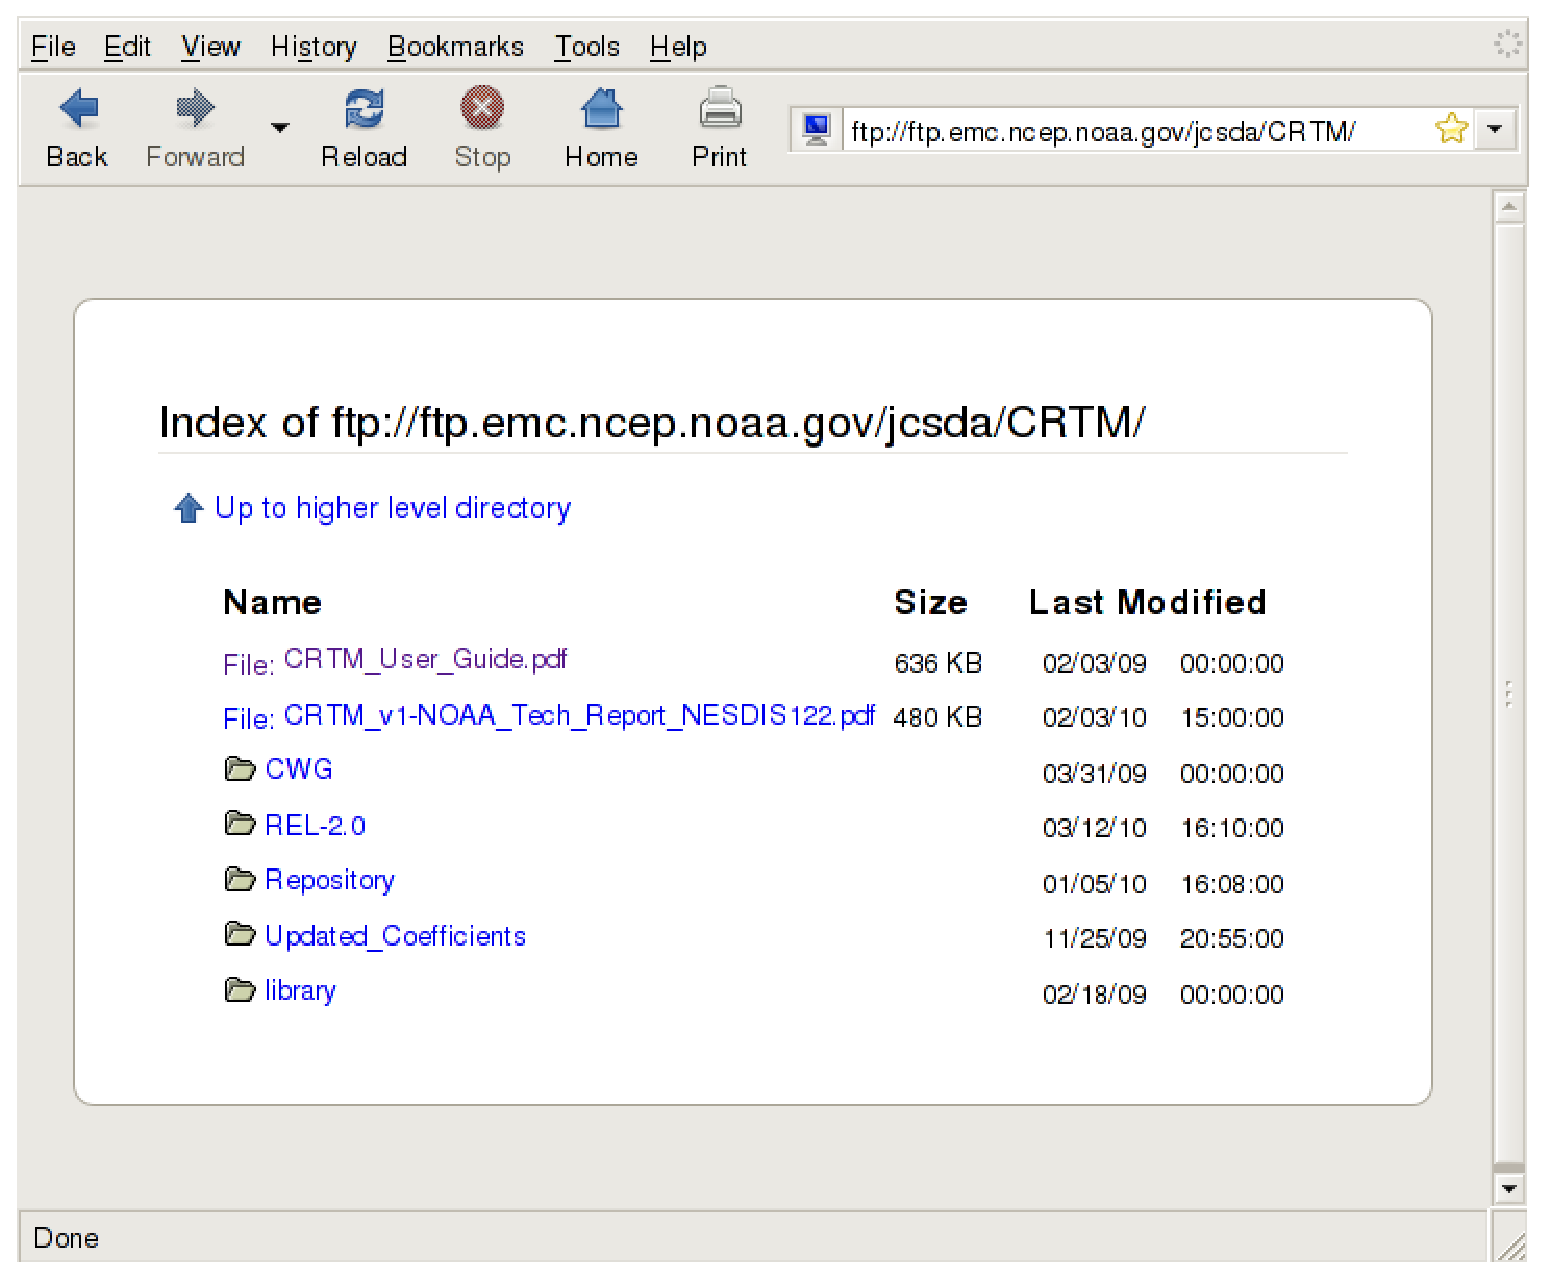
\includegraphics[scale=0.5]{graphics/Get/CRTM_ftp_site.eps}
  \caption{The CRTM ftp site contents (as on Jan.29, 2009)}
  \label{fig:ftp_site}
\end{figure}

\section{How to build the CRTM library}
%======================================

\chapter{How to use the CRTM library}
%====================================

error status description

\section{Quick Start}
%====================

Quick start guide via examples. Refer to the following sections for more information about the structures and interfaces.

The first thing you need to do is identify what sensors you want to use. The list of supported sensors, along with their associated \texttt{Sensor\_Id}'s, are shown in appendix BLAH




\section{Interface Descriptions}
%===============================

\subsection{CRTM Initialisation}
%-------------------------------

\begin{figure}[htp]
  \centering
  \doublebox{
  \begin{minipage}[b]{6.5in}
    \begin{ttfamily}
      \begin{verbatim}
  FUNCTION CRTM_Init( ChannelInfo      , &  ! Output, N
                      Sensor_ID        , &  ! Optional input, N
                      CloudCoeff_File  , &  ! Optional input
                      AerosolCoeff_File, &  ! Optional input
                      EmisCoeff_File   , &  ! Optional input
                      File_Path        , &  ! Optional input
                      Quiet            , &  ! Optional input
                      Process_ID       , &  ! Optional input
                      Output_Process_ID, &  ! Optional input
                      RCS_Id           , &  ! Revision control
                      Message_Log      ) &  ! Error messaging
                    RESULT( Error_Status )

    ! Arguments
    TYPE(CRTM_ChannelInfo_type), INTENT(IN OUT) :: ChannelInfo(:)  ! N
    CHARACTER(*),      OPTIONAL, INTENT(IN)     :: Sensor_ID(:)    ! N
    CHARACTER(*),      OPTIONAL, INTENT(IN)     :: CloudCoeff_File
    CHARACTER(*),      OPTIONAL, INTENT(IN)     :: AerosolCoeff_File
    CHARACTER(*),      OPTIONAL, INTENT(IN)     :: EmisCoeff_File
    CHARACTER(*),      OPTIONAL, INTENT(IN)     :: File_Path
    INTEGER     ,      OPTIONAL, INTENT(IN)     :: Quiet
    INTEGER     ,      OPTIONAL, INTENT(IN)     :: Process_ID
    INTEGER     ,      OPTIONAL, INTENT(IN)     :: Output_Process_ID
    CHARACTER(*),      OPTIONAL, INTENT(OUT)    :: RCS_Id
    CHARACTER(*),      OPTIONAL, INTENT(IN)     :: Message_Log
    ! Function result
    INTEGER :: Error_Status
      \end{verbatim}
    \end{ttfamily}
    \centering
    \begin{tabular}{c|c|c|c}
      \textbf{Argument} & \textbf{Description}                     & \textbf{Rank}   & \textbf{Intent} \\
      \hline\hline
      ChannelInfo        & Sensor and channel info structure       & n\_Sensors (N)  & IN OUT      \\
      \hline
      Sensor\_Id         & Sensor identification string            & n\_Sensors (N)  & IN      \\
      \hline
      CloudCoeff\_File   & Cloud optical property LUT filename     & Scalar          & IN      \\
      \hline
      AerosolCoeff\_File & Aerosol optical property LUT filename   & Scalar          & IN      \\
      \hline
      EmisCoeff\_File    & IR sea surface emissivity LUT filename  & Scalar          & IN      \\
      \hline
      File\_Path         & Path to *Coeff files                    & Scalar          & IN      \\
      \hline
      Quiet              & Keyword to control information message output & Scalar         & IN      \\
      \hline
      Process\_Id        & MPI process Id                          & Scalar          & IN      \\
      \hline
      Output\_Process\_Id & MPI process Id for message output      & Scalar          & IN      \\
      \hline
      RCS\_Id            & Version control ID for the module      & Scalar           & OUT     \\
      \hline
      Message\_Log       & Log message filename                   & Scalar           & IN      \\
    \end{tabular}
  \end{minipage}
  }
  \caption{CRTM Initialisation interface and argument description.}
  \label{fig:init_interface}
\end{figure}

\subsection{Forward Model}
%-------------------------

\begin{figure}[htp]
  \centering
  \doublebox{
  \begin{minipage}[b]{6.5in}
    \begin{ttfamily}
      \begin{verbatim}
  FUNCTION CRTM_Forward( Atmosphere  , &  ! Input, M
                         Surface     , &  ! Input, M    
                         GeometryInfo, &  ! Input, M    
                         ChannelInfo , &  ! Input, N
                         RTSolution  , &  ! Output, L x M   
                         Options     , &  ! Optional input, M    
                         RCS_Id      , &  ! Revision control
                         Message_Log ) &  ! Error messaging
                       RESULT( Error_Status )
    ! Arguments
    TYPE(CRTM_Atmosphere_type),        INTENT(IN)     :: Atmosphere(:)     ! M
    TYPE(CRTM_Surface_type),           INTENT(IN)     :: Surface(:)        ! M
    TYPE(CRTM_GeometryInfo_type),      INTENT(IN OUT) :: GeometryInfo(:)   ! M
    TYPE(CRTM_ChannelInfo_type),       INTENT(IN)     :: ChannelInfo(:)    ! N 
    TYPE(CRTM_RTSolution_type),        INTENT(IN OUT) :: RTSolution(:,:)   ! L x M
    TYPE(CRTM_Options_type), OPTIONAL, INTENT(IN)     :: Options(:)        ! M
    CHARACTER(*),            OPTIONAL, INTENT(OUT)    :: RCS_Id
    CHARACTER(*),            OPTIONAL, INTENT(IN)     :: Message_Log
    ! Function result
    INTEGER :: Error_Status
      \end{verbatim}
    \end{ttfamily}
    \centering
    \begin{tabular}{c|c|c|c}
      \textbf{Argument} & \textbf{Description}                    & \textbf{Rank}    & \textbf{Intent} \\
      \hline\hline
      Atmosphere         & Atmospheric state                      & n\_Profiles (M)  & IN      \\
      \hline
      Surface            & Surface state                          & n\_Profiles (M)  & IN      \\
      \hline
      GeometryInfo       & Geometry information (e.g. angles)     & n\_Profiles (M)  & IN      \\
      \hline
      ChannelInfo        & Sensor channel information             & n\_Sensors (N)   & IN      \\
      \hline
      RTSolution         & Radiative transfer solution            & n\_Channels x n\_Profiles                 & IN OUT  \\
      \hline
      Options            & Structure for optional input           & n\_Profiles (M)  & IN      \\
      \hline
      RCS\_Id            & Version control ID for the module      & Scalar           & OUT     \\
      \hline
      Message\_Log       & Log message filename                   & Scalar           & IN      \\
    \end{tabular}
  \end{minipage}
  }
  \caption{CRTM Forward model interface and argument description.}
  \label{fig:fwd_interface}
\end{figure}


\subsection{K-Matrix Model}
%--------------------------

\begin{figure}[htp]
  \centering
  \doublebox{
  \begin{minipage}[b]{6.5in}
    \begin{ttfamily}
      \begin{verbatim}
  FUNCTION CRTM_K_Matrix( Atmosphere  , &  ! FWD Input, M
                          Surface     , &  ! FWD Input, M
                          RTSolution_K, &  ! K   Input, L x M   
                          GeometryInfo, &  ! Input, M
                          ChannelInfo , &  ! Input, N  
                          Atmosphere_K, &  ! K   Output, L x M
                          Surface_K   , &  ! K   Output, L x M
                          RTSolution  , &  ! FWD Output, L x M
                          Options     , &  ! Optional FWD input, M
                          RCS_Id      , &  ! Revision control
                          Message_Log ) &  ! Error messaging
                        RESULT( Error_Status )
    ! Arguments
    TYPE(CRTM_Atmosphere_type)       , INTENT(IN)     :: Atmosphere(:)     ! M
    TYPE(CRTM_Surface_type)          , INTENT(IN)     :: Surface(:)        ! M
    TYPE(CRTM_RTSolution_type)       , INTENT(IN OUT) :: RTSolution_K(:,:) ! L x M
    TYPE(CRTM_GeometryInfo_type)     , INTENT(IN OUT) :: GeometryInfo(:)   ! M
    TYPE(CRTM_ChannelInfo_type)      , INTENT(IN)     :: ChannelInfo(:)    ! N
    TYPE(CRTM_Atmosphere_type)       , INTENT(IN OUT) :: Atmosphere_K(:,:) ! L x M
    TYPE(CRTM_Surface_type)          , INTENT(IN OUT) :: Surface_K(:,:)    ! L x M
    TYPE(CRTM_RTSolution_type)       , INTENT(IN OUT) :: RTSolution(:,:)   ! L x M
    TYPE(CRTM_Options_type), OPTIONAL, INTENT(IN)     :: Options(:)        ! M
    CHARACTER(*),            OPTIONAL, INTENT(OUT)    :: RCS_Id
    CHARACTER(*),            OPTIONAL, INTENT(IN)     :: Message_Log
    ! Function result
    INTEGER :: Error_Status
      \end{verbatim}
    \end{ttfamily}
    \centering
    \begin{tabular}{c|c|c|c}
      \textbf{Argument} & \textbf{Description}                    & \textbf{Rank}    & \textbf{Intent} \\
      \hline\hline
      Atmosphere         & Atmospheric state                      & n\_Profiles (M)  & IN      \\
      \hline
      Surface            & Surface state                          & n\_Profiles (M)  & IN      \\
      \hline
      RTSolution\_K      & Adjoint radiative transfer solution    & n\_Channels (L) x n\_Profiles (M) & IN OUT  \\
      \hline
      GeometryInfo       & Geometry information (e.g. angles)     & n\_Profiles (M)  & IN      \\
      \hline
      ChannelInfo        & Sensor channel information             & n\_Sensors (N)   & IN      \\
      \hline
      Atmosphere\_K      & Atmospheric state Jacobians            & n\_Channels (L) x n\_Profiles (M) & IN OUT  \\
      \hline
      Surface\_K         & Surface state Jacobians                & n\_Channels (L) x n\_Profiles (M) & IN OUT  \\
      \hline
      RTSolution         & Radiative transfer solution            & n\_Channels (L) x n\_Profiles (M) & IN OUT      \\
      \hline
      Options            & Structure for optional input           & n\_Profiles (M)  & IN      \\
      \hline
      RCS\_Id            & Version control ID for the module      & Scalar           & OUT     \\
      \hline
      Message\_Log       & Log message filename                   & Scalar           & IN      \\
    \end{tabular}
  \end{minipage}
  }
  \caption{CRTM K-Matrix model interface and argument description.}
  \label{fig:k_interface}
\end{figure}


\subsection{CRTM Destruction}
%----------------------------

\begin{figure}[htp]
  \centering
  \doublebox{
  \begin{minipage}[b]{6.5in}
    \begin{ttfamily}
      \begin{verbatim}
  FUNCTION CRTM_Destroy( ChannelInfo , &  ! Output
                         Process_ID  , &  ! Optional input
                         RCS_Id      , &  ! Revision control
                         Message_Log ) &  ! Error messaging
                       RESULT ( Error_Status )
    ! Arguments
    TYPE(CRTM_ChannelInfo_type), INTENT(IN OUT) :: ChannelInfo(:)
    INTEGER     ,      OPTIONAL, INTENT(IN)     :: Process_ID
    CHARACTER(*),      OPTIONAL, INTENT(OUT)    :: RCS_Id
    CHARACTER(*),      OPTIONAL, INTENT(IN)     :: Message_Log
    ! Function result
    INTEGER :: Error_Status
      \end{verbatim}
    \end{ttfamily}
    \centering
    \begin{tabular}{c|c|c|c}
      \textbf{Argument} & \textbf{Description}                     & \textbf{Rank}   & \textbf{Intent} \\
      \hline\hline
      ChannelInfo        & Sensor and channel info structure       & n\_Sensors (N)  & IN OUT      \\
      \hline
      Process\_Id        & MPI process Id                          & Scalar          & IN      \\
      \hline
      RCS\_Id            & Version control ID for the module      & Scalar           & OUT     \\
      \hline
      Message\_Log       & Log message filename                   & Scalar           & IN      \\
    \end{tabular}
  \end{minipage}
  }
  \caption{CRTM Destruction interface and argument description.}
  \label{fig:destroy_interface}
\end{figure}


\section{Filling input data structures}
%======================================

\begin{figure}[htp]
  \centering
  \input{graphics/gInfo/sensor_scan_angle.pstex_t}
  \caption{Definition of \GeometryInfo{} sensor scan angle component.}
  \label{fig:gInfo_sensor_scan_angle}
\end{figure}

\begin{figure}[htp]
  \centering
  \input{graphics/gInfo/sensor_zenith_angle.pstex_t}
  \caption{Definition of \GeometryInfo{} sensor zenith angle component.}
  \label{fig:gInfo_sensor_zenith_angle}
\end{figure}

\begin{figure}[htp]
  \centering
  \input{graphics/gInfo/sensor_azimuth_angle.pstex_t}
  \caption{Definition of \GeometryInfo{} sensor azimuth angle component.}
  \label{fig:gInfo_sensor_azimuth_angle}
\end{figure}

\begin{figure}[htp]
  \centering
  \input{graphics/gInfo/source_zenith_angle.pstex_t}
  \caption{Definition of \GeometryInfo{} source zenith angle component.}
  \label{fig:gInfo_source_zenith_angle}
\end{figure}

\begin{figure}[htp]
  \centering
  \input{graphics/gInfo/source_azimuth_angle.pstex_t}
  \caption{Definition of \GeometryInfo{} source azimuth angle component.}
  \label{fig:gInfo_source_azimuth_angle}
\end{figure}



% The appendices
%===============
\begin{appendix}
  \chapter{Structure definitions}
%==============================

\section{\Atmosphere{} Structure}
%================================
\label{sec:atmosphere_structure}

\begin{figure}[htp]
  \centering
  \doublebox{
  \begin{minipage}[b]{6.5in}
    \begin{ttfamily}
      \begin{verbatim}
  TYPE :: CRTM_Atmosphere_type
    ! Dimension values
    INTEGER :: n_Layers     = 0  ! K dimension
    INTEGER :: n_Absorbers  = 0  ! J dimension
    INTEGER :: n_Clouds     = 0  ! Nc dimension
    INTEGER :: n_Aerosols   = 0  ! Na dimension
    ! Number of added layers
    INTEGER :: n_Added_Layers = 0
    ! Climatology model associated with the profile
    INTEGER :: Climatology = INVALID_MODEL
    ! Absorber ID and units
    INTEGER, POINTER :: Absorber_ID(:)    => NULL() ! J
    INTEGER, POINTER :: Absorber_Units(:) => NULL() ! J
    ! Profile LEVEL and LAYER quantities
    REAL(fp), POINTER :: Level_Pressure(:) => NULL()  ! 0:K
    REAL(fp), POINTER :: Pressure(:)       => NULL()  ! K
    REAL(fp), POINTER :: Temperature(:)    => NULL()  ! K
    REAL(fp), POINTER :: Absorber(:,:)     => NULL()  ! K x J
    ! Clouds associated with each profile
    TYPE(CRTM_Cloud_type),   POINTER :: Cloud(:)   => NULL()  ! Nc
    ! Aerosols associated with each profile
    TYPE(CRTM_Aerosol_type), POINTER :: Aerosol(:) => NULL()  ! Na
  END TYPE CRTM_Atmosphere_type\end{verbatim}
    \end{ttfamily}
  \end{minipage}
  }
  \caption{CRTM \Atmosphere{} structure definition.}
  \label{fig:atmosphere_structure}
\end{figure}

% Atmosphere component description table
\begin{table}[htp]
  \centering
  \begin{tabular}{|l|p{7cm}|c|c|}
    \hline
    \sffamily\textbf{Component} & \sffamily\textbf{Description} & \sffamily\textbf{Units} & \sffamily\textbf{Dimensions} \\
    \hline\hline
    \texttt{n\_Layers} & Number of atmospheric profile layers (\texttt{K}) & N/A & Scalar \\
    \texttt{n\_Absorbers} & Number of atmospheric absorbers (\texttt{J}) & N/A & Scalar \\
    \texttt{n\_Clouds} & Number of clouds (\texttt{Nc}) & N/A & Scalar \\
    \texttt{n\_Aerosols} & Number of aerosols (\texttt{Na}) & N/A & Scalar \\
    \texttt{n\_Added\_Layers} & Number of layers added so as to extend the input profile to nominal TOA  & N/A & Scalar \\
    \texttt{Climatology} & Climatology of the profile (see table \ref{tab:climatology}) & N/A & Scalar \\
    \texttt{Absorber\_Id} & Gaseous absorber identifiers (see table \ref{tab:absorber_id}) & N/A & \texttt{J}\\
    \texttt{Absorber\_Units} & Gaseous absorber amount units (see table \ref{tab:absorber_units}) & N/A & \texttt{J}\\
    \texttt{Level\_Pressure} & Interface pressures of the profile layers & hPa & \texttt{0:K} \\
    \texttt{Pressure} & Average layer pressure & hPa & \texttt{K} \\
    \texttt{Temperatures} & Layer temperatures & Kelvin & \texttt{K} \\
    \texttt{Absorbers} & Layer absorber amount & Variable & \texttt{K} $\times$ \texttt{J}\\
    \texttt{Cloud} & Cloud structure array & N/A & \texttt{Nc}\\
    \texttt{Aerosol} & Aerosol structure array & N/A & \texttt{Na}\\
    \hline
  \end{tabular}
  \caption{CRTM \Atmosphere{} structure component description.}
  \label{tab:atmosphere_structure}
\end{table}

% Climatology table
\begin{table}[htp]
  \centering
  \begin{tabular}{|c|c|}
    \hline
    \sffamily\textbf{Climatology Type} & \sffamily\textbf{Parameter} \\
    \hline\hline
             Tropical          &  \texttt{TROPICAL}\\              
        Midlatitude summer     &  \texttt{MIDLATITUDE\_SUMMER}\\
        Midlatitude winter     &  \texttt{MIDLATITUDE\_WINTER}\\
         Subarctic summer      &  \texttt{SUBARCTIC\_SUMMER}\\
         Subarctic winter      &  \texttt{SUBARCTIC\_WINTER}\\
     U.S. Standard Atmosphere  &  \texttt{US\_STANDARD\_ATMOSPHERE}\\
    \hline 
  \end{tabular}
  \caption{CRTM \Atmosphere{} structure valid \texttt{Climatology} definitions. The same set as defined for LBLRTM is used.}
  \label{tab:climatology}
\end{table}

% Absorber id table
\begin{table}
  \centering
  \begin{tabular}{|c|c||c|c|}
    \hline
    \sffamily\textbf{Molecule} & \sffamily\textbf{Parameter} & \sffamily\textbf{Molecule} & \sffamily\textbf{Parameter}\\
    \hline\hline
     H\subscript{2}O  & \texttt{H2O\_ID}  &    HI & \texttt{   HI\_ID}\\
     CO\subscript{2}  & \texttt{CO2\_ID}  &   ClO & \texttt{  ClO\_ID}\\
     O\subscript{3}   & \texttt{O3\_ID}   &   OCS & \texttt{  OCS\_ID}\\
     N\subscript{2}O  & \texttt{N2O\_ID}  &  H\subscript{2}CO & \texttt{ H2CO\_ID}\\
     CO               & \texttt{CO\_ID}   &  HOCl & \texttt{ HOCl\_ID}\\
     CH\subscript{4}  & \texttt{CH4\_ID}  &    N\subscript{2} & \texttt{   N2\_ID}\\
     O\subscript{2}   & \texttt{O2\_ID}   &   HCN & \texttt{  HCN\_ID}\\
     NO               & \texttt{NO\_ID}   &  CH\subscript{3}l & \texttt{ CH3l\_ID}\\
     SO\subscript{2}  & \texttt{SO2\_ID}  &  H\subscript{2}O\subscript{2} & \texttt{ H2O2\_ID}\\
     NO\subscript{2}  & \texttt{NO2\_ID}  &  C\subscript{2}H\subscript{2} & \texttt{ C2H2\_ID}\\
     NH\subscript{3}  & \texttt{NH3\_ID}  &  C\subscript{2}H\subscript{6} & \texttt{ C2H6\_ID}\\
     HNO\subscript{3} & \texttt{HNO3\_ID} &   PH\subscript{3} & \texttt{  PH3\_ID}\\
     OH               & \texttt{OH\_ID}   &  COF\subscript{2} & \texttt{ COF2\_ID}\\
     HF               & \texttt{HF\_ID}   &   SF\subscript{6} & \texttt{  SF6\_ID}\\
     HCl              & \texttt{HCl\_ID}  &   H\subscript{2}S & \texttt{  H2S\_ID}\\
     HBr              & \texttt{HBr\_ID}  & HCOOH & \texttt{HCOOH\_ID}\\
    \hline
  \end{tabular}
  \caption{CRTM \Atmosphere{} structure valid \texttt{Absorber\_ID} definitions. The same molecule set as defined for HITRAN is used.}
  \label{tab:absorber_id}
\end{table}

% Absorber units table
\begin{table}
  \centering
  \begin{tabular}{|c|c|}
    \hline
    \sffamily\textbf{Units} & \sffamily\textbf{Parameter} \\
    \hline\hline
     Volume mixing ratio, ppmv                       & \texttt{VOLUME\_MIXING\_RATIO\_UNITS} \\
     Number density, cm$^{-3}$                       & \texttt{NUMBER\_DENSITY\_UNITS} \\
     Mass mixing ratio, g/kg                         & \texttt{MASS\_MIXING\_RATIO\_UNITS} \\
     Mass density, g.m$^{-3}$                        & \texttt{MASS\_DENSITY\_UNITS} \\
     Partial pressure, hPa                           & \texttt{PARTIAL\_PRESSURE\_UNITS} \\
     Dewpoint temperature, K  \textbf{(H$\mathbf{_2}$O ONLY)} & \texttt{DEWPOINT\_TEMPERATURE\_K\_UNITS} \\
     Dewpoint temperature, C  \textbf{(H$\mathbf{_2}$O ONLY)} & \texttt{DEWPOINT\_TEMPERATURE\_C\_UNITS} \\
     Relative humidity, \%    \textbf{(H$\mathbf{_2}$O ONLY)} & \texttt{RELATIVE\_HUMIDITY\_UNITS} \\
     Specific amount, g/g                            & \texttt{SPECIFIC\_AMOUNT\_UNITS} \\
     Integrated path, mm                             & \texttt{INTEGRATED\_PATH\_UNITS} \\
    \hline
  \end{tabular}
  \caption{CRTM \Atmosphere{} structure valid \texttt{Absorber\_Units} definitions. The same set as defined for LBLRTM is used.}
  \label{tab:absorber_units}
\end{table}

\subsection{\Cloud{} Structure}
%------------------------------
\label{sec:cloud_structure}

\begin{figure}[htp]
  \centering
  \doublebox{
  \begin{minipage}[b]{6.5in}
    \begin{ttfamily}
      \begin{verbatim}
  TYPE :: CRTM_Cloud_type
    ! Dimension values
    INTEGER :: n_Layers = 0  ! K dimension.
    ! Number of added layers
    INTEGER :: n_Added_Layers = 0
    ! Cloud type
    INTEGER :: Type = NO_CLOUD
    ! Cloud state variables
    REAL(fp), POINTER :: Effective_Radius(:)   => NULL() ! K
    REAL(fp), POINTER :: Effective_Variance(:) => NULL() ! K
    REAL(fp), POINTER :: Water_Content(:)      => NULL() ! K
  END TYPE CRTM_Cloud_type\end{verbatim}
    \end{ttfamily}
  \end{minipage}
  }
  \caption{CRTM \Cloud{} structure definition.}
  \label{fig:cloud_structure}
\end{figure}

% Cloud component description table
\begin{table}[htp]
  \centering
  \begin{tabular}{|l|p{7cm}|c|c|}
    \hline
    \sffamily\textbf{Component} & \sffamily\textbf{Description} & \sffamily\textbf{Units} & \sffamily\textbf{Dimensions} \\
    \hline\hline
    \texttt{n\_Layers} & Number of atmospheric profile layers (\texttt{K}) & N/A & Scalar \\
    \texttt{n\_Added\_Layers} & Number of layers added so as to extend the input profile to nominal TOA  & N/A & Scalar \\
    \texttt{Type} & Type of cloud (see table \ref{tab:cloud_type}) & N/A & Scalar \\
    \texttt{Effective\_Radius} & Cloud particle $r_{eff}$ profile & \micron & \texttt{K} \\
    \texttt{Effective\_Variance} & Cloud particle $\sigma_{eff}$ profile & \micron$^2$ & \texttt{K} \\
    \texttt{Water\_Content} & Cloud water content profile & kg.m$^{-2}$ & \texttt{K} \\
    \hline
  \end{tabular}
  \caption{CRTM \Cloud{} structure component description.}
  \label{tab:cloud_structure}
\end{table}

% Cloud type table
\begin{table}
  \centering
  \begin{tabular}{|c|c|}
    \hline
    \sffamily\textbf{Cloud Type} & \sffamily\textbf{Parameter} \\
    \hline\hline
     Water   & \texttt{WATER\_CLOUD}\\
     Ice     & \texttt{ICE\_CLOUD}\\
     Rain    & \texttt{RAIN\_CLOUD}\\
     Snow    & \texttt{SNOW\_CLOUD}\\
     Graupel & \texttt{GRAUPEL\_CLOUD}\\
     Hail    & \texttt{HAIL\_CLOUD}\\
    \hline
  \end{tabular}
  \caption{CRTM \Cloud{} structure valid \texttt{Type} definitions.}
  \label{tab:cloud_type}
\end{table}


\subsection{\Aerosol{} Structure}
%--------------------------------
\label{aerosol_structdef}


\begin{figure}[htp]
  \centering
  \doublebox{
  \begin{minipage}[b]{6.5in}
    \begin{ttfamily}
      \begin{verbatim}
  TYPE :: CRTM_Aerosol_type
    ! Dimensions
    INTEGER :: n_Layers = 0  ! K dimension
    ! Number of added layers    
    INTEGER :: n_Added_Layers = 0
    ! Aerosol type
    INTEGER :: Type = NO_AEROSOL
    ! Aerosol state variables
    REAL(fp), POINTER :: Effective_Radius(:) => NULL()  ! K
    REAL(fp), POINTER :: Concentration(:)    => NULL()  ! K
  END TYPE CRTM_Aerosol_type\end{verbatim}
    \end{ttfamily}
  \end{minipage}
  }
  \caption{CRTM \Aerosol{} structure definition.}
  \label{fig:aerosol_structure}
\end{figure}

% Aerosol component description table
\begin{table}[htp]
  \centering
  \begin{tabular}{|l|p{7cm}|c|c|}
    \hline
    \sffamily\textbf{Component} & \sffamily\textbf{Description} & \sffamily\textbf{Units} & \sffamily\textbf{Dimensions} \\
    \hline\hline
    \texttt{n\_Layers} & Number of atmospheric profile layers (\texttt{K}) & N/A & Scalar \\
    \texttt{n\_Added\_Layers} & Number of layers added so as to extend the input profile to nominal TOA  & N/A & Scalar \\
    \texttt{Type} & Type of Aerosol (see table \ref{tab:aerosol_type}) & N/A & Scalar \\
    \texttt{Effective\_Radius} & Aerosol particle $r_{eff}$ profile & \micron & \texttt{K} \\
    \texttt{Concentration} & Aerosol concentration profile & kg.m$^{-2}$ & \texttt{K} \\
    \hline
  \end{tabular}
  \caption{CRTM \Aerosol{} structure component description.}
  \label{tab:aerosol_structure}
\end{table}

% Aerosol type table
\begin{table}
  \centering
  \begin{tabular}{|c|c|}
    \hline
    \sffamily\textbf{Aerosol Type} & \sffamily\textbf{Parameter} \\
    \hline\hline
           Dust         &  \texttt{DUST\_AEROSOL}\\
       Sea salt SSAM\footnote{SSAM $\equiv$ sea salt accumulation mode, $r_{eff}\sim$0.5-5.0\micron.} &  \texttt{SEASALT\_SSAM\_AEROSOL}\\
       Sea salt SSCM\footnote{SSCM $\equiv$ sea salt coarse mode, $r_{eff}\sim$5.0-30\micron} &  \texttt{SEASALT\_SSCM\_AEROSOL}\\
     Dry organic carbon &  \texttt{DRY\_ORGANIC\_CARBON\_AEROSOL}\\
     Wet organic carbon &  \texttt{WET\_ORGANIC\_CARBON\_AEROSOL}\\
      Dry black carbon  &  \texttt{DRY\_BLACK\_CARBON\_AEROSOL}\\
      Wet black carbon  &  \texttt{WET\_BLACK\_CARBON\_AEROSOL}\\
          Sulfate       &  \texttt{SULFATE\_AEROSOL}\\
    \hline
  \end{tabular}
  \caption{CRTM \Aerosol{} structure valid \texttt{Type} definitions.}
  \label{tab:aerosol_type}
\end{table}



\section{\Surface{} Structure}
%=============================
\label{surface_structdef}

\begin{figure}[htp]
  \centering
  \doublebox{
  \begin{minipage}[b]{6.5in}
    \begin{ttfamily}
      \begin{verbatim}
  TYPE :: CRTM_Surface_type
    ! Dimension values
    INTEGER :: n_Sensors    = 0  ! N dimension
    ! Gross type of surface determined by coverage
    REAL(fp) :: Land_Coverage  = ZERO
    REAL(fp) :: Water_Coverage = ZERO
    REAL(fp) :: Snow_Coverage  = ZERO
    REAL(fp) :: Ice_Coverage   = ZERO
    ! Surface type independent data
    REAL(fp) :: Wind_Speed     = DEFAULT_WIND_SPEED
    REAL(fp) :: Wind_Direction = DEFAULT_WIND_DIRECTION
    ! Land surface type data
    INTEGER  :: Land_Type             = DEFAULT_LAND_TYPE
    REAL(fp) :: Land_Temperature      = DEFAULT_LAND_TEMPERATURE
    REAL(fp) :: Soil_Moisture_Content = DEFAULT_SOIL_MOISTURE_CONTENT
    REAL(fp) :: Canopy_Water_Content  = DEFAULT_CANOPY_WATER_CONTENT
    REAL(fp) :: Vegetation_Fraction   = DEFAULT_VEGETATION_FRACTION
    REAL(fp) :: Soil_Temperature      = DEFAULT_SOIL_TEMPERATURE
    ! Water type data
    INTEGER  :: Water_Type        = DEFAULT_WATER_TYPE
    REAL(fp) :: Water_Temperature = DEFAULT_WATER_TEMPERATURE
    REAL(fp) :: Salinity          = DEFAULT_SALINITY
    ! Snow surface type data
    INTEGER  :: Snow_Type        = DEFAULT_SNOW_TYPE
    REAL(fp) :: Snow_Temperature = DEFAULT_SNOW_TEMPERATURE
    REAL(fp) :: Snow_Depth       = DEFAULT_SNOW_DEPTH
    REAL(fp) :: Snow_Density     = DEFAULT_SNOW_DENSITY
    REAL(fp) :: Snow_Grain_Size  = DEFAULT_SNOW_GRAIN_SIZE
    ! Ice surface type data
    INTEGER  :: Ice_Type        = DEFAULT_ICE_TYPE
    REAL(fp) :: Ice_Temperature = DEFAULT_ICE_TEMPERATURE
    REAL(fp) :: Ice_Thickness   = DEFAULT_ICE_THICKNESS
    REAL(fp) :: Ice_Density     = DEFAULT_ICE_DENSITY
    REAL(fp) :: Ice_Roughness   = DEFAULT_ICE_ROUGHNESS
    ! SensorData containing channel brightness temperatures
    TYPE(CRTM_SensorData_type) :: SensorData  ! N
  END TYPE CRTM_Surface_type\end{verbatim}
    \end{ttfamily}
  \end{minipage}
  }
  \caption{CRTM \Surface{} structure definition.}
  \label{fig:surface_structure}
\end{figure}

\begin{table}[htp]
  \centering
  \begin{tabular}{|l|p{7cm}|c|c|}
    \hline
    \sffamily\textbf{Component} & \sffamily\textbf{Description} & \sffamily\textbf{Units} & \sffamily\textbf{Dimensions} \\
    \hline\hline
    \texttt{n\_Sensors} & The number of sensors for which data is provided inside the SensorData structure & N/A & Scalar \\
    \hline
    \texttt{Land\_Coverage}  & Fraction of the FOV that is land surface & N/A & Scalar \\
    \texttt{Water\_Coverage} & Fraction of the FOV that is water surface & N/A & Scalar \\
    \texttt{Snow\_Coverage}  & Fraction of the FOV that is snow surface & N/A & Scalar \\
    \texttt{Ice\_Coverage}   & Fraction of the FOV that is ice surface & N/A & Scalar \\
    \hline
    \texttt{Wind\_Speed}     & Surface wind speed & m.s$^{-1}$ & Scalar \\
    \texttt{Wind\_Direction} & Surface wind direction & deg. E from N & Scalar \\
    \hline
    \texttt{Land\_Type}              & Land surface type & N/A & Scalar \\
    \texttt{Land\_Temperature}       & Land surface temperature & Kelvin & Scalar \\
    \texttt{Soil\_Moisture\_Content} & Volumetric water content of the soil & g.cm$^{-3}$ & Scalar \\
    \texttt{Canopy\_Water\_Content}  & Gravimetric water content of the canopy & g.cm$^{-3}$ & Scalar \\
    \texttt{Vegetation\_Fraction}    & Vegetation fraction of the surface & \% & Scalar \\
    \texttt{Soil\_Temperature}       & Soil temperature & Kelvin & Scalar \\
    \hline
    \texttt{Water\_Type}        & Water surface type & N/A & Scalar \\
    \texttt{Water\_Temperature} & Water surface temperature & Kelvin & Scalar \\
    \texttt{Salinity}           & Water salinity & \textperthousand & Scalar \\
    \hline
    \texttt{Snow\_Type}        & Snow surface type & N/A & Scalar \\ 
    \texttt{Snow\_Temperature} & Snow surface temperature & Kelvin & Scalar \\ 
    \texttt{Snow\_Depth}       & Snow depth & mm & Scalar \\ 
    \texttt{Snow\_Density}     & Snow density & g.m$^{-3}$ & Scalar \\ 
    \texttt{Snow\_Grain\_Size} & Snow grain size & mm & Scalar \\ 
    \hline
    \texttt{Ice\_Type}        & Ice surface type & N/A & Scalar \\ 
    \texttt{Ice\_Temperature} & Ice surface temperature & Kelvin & Scalar \\ 
    \texttt{Ice\_Thickness}   & Thickness of ice & mm & Scalar \\ 
    \texttt{Ice\_Density}     & Density of ice & g.m$^{-3}$ & Scalar \\ 
    \texttt{Ice\_Roughness}   & Measure of the surface roughness of the ice & N/A & Scalar \\ 
    \hline
    \texttt{SensorData} & Satellite sensor data required for some surface emissivity algorithms & N/A & Scalar \\ 
    \hline
  \end{tabular}
  \caption{CRTM \Surface{} structure component description.}
  \label{tav:surface_structure}
\end{table}

% Default surface value table
\begin{table}[htp]
  \centering
  \begin{tabular}{|c|c|c|}
    \hline
    \sffamily\textbf{Parameter} & \sffamily\textbf{Value}  & \sffamily\textbf{Units} \\
    \hline\hline
    \multicolumn{3}{|c|}{Surface type independent data}\\
    \hline
    \texttt{DEFAULT\_WIND\_SPEED}             & 5.0        & m.s$^{-1}$\\
    \texttt{DEFAULT\_WIND\_DIRECTION}         & 0.0        & deg. E from N\\
    \hline
    \multicolumn{3}{|c|}{Land surface type data}\\
    \hline
    \texttt{DEFAULT\_LAND\_TYPE}              & \texttt{GRASS\_SOIL}& N/A \\
    \texttt{DEFAULT\_LAND\_TEMPERATURE}       & 283.0      & K\\
    \texttt{DEFAULT\_SOIL\_MOISTURE\_CONTENT} & 0.05       & g.cm$^{-3}$\\
    \texttt{DEFAULT\_CANOPY\_WATER\_CONTENT}  & 0.05       & g.cm$^{-3}$\\
    \texttt{DEFAULT\_VEGETATION\_FRACTION}    & 0.3        & 30\%\\
    \texttt{DEFAULT\_SOIL\_TEMPERATURE}       & 283.0      & K\\
    \hline
    \multicolumn{3}{|c|}{Water type data}\\
    \hline
    \texttt{DEFAULT\_WATER\_TYPE}             & \texttt{SEA\_WATER} & N/A\\
    \texttt{DEFAULT\_WATER\_TEMPERATURE}      & 283.0      & K\\
    \texttt{DEFAULT\_SALINITY}                & 33.0       & ppmv\\
    \hline
    \multicolumn{3}{|c|}{Snow surface type data}\\
    \hline
    \texttt{DEFAULT\_SNOW\_TYPE}              & \texttt{NEW\_SNOW}  & N/A\\
    \texttt{DEFAULT\_SNOW\_TEMPERATURE}       & 263.0      & K\\
    \texttt{DEFAULT\_SNOW\_DEPTH}             & 50.0       & mm\\
    \texttt{DEFAULT\_SNOW\_DENSITY}           & 0.2        & g.cm$^{-3}$\\
    \texttt{DEFAULT\_SNOW\_GRAIN\_SIZE}       & 2.0        & mm\\
    \hline
    \multicolumn{3}{|c|}{Ice surface type data}\\
    \hline
    \texttt{DEFAULT\_ICE\_TYPE}               & \texttt{FRESH\_ICE} & N/A\\
    \texttt{DEFAULT\_ICE\_TEMPERATURE}        & 263.0      & K\\
    \texttt{DEFAULT\_ICE\_THICKNESS}          & 10.0       & mm\\
    \texttt{DEFAULT\_ICE\_DENSITY}            & 0.9        & g.cm$^{-3}$\\
    \texttt{DEFAULT\_ICE\_ROUGHNESS}          & ZERO       & N/A\\
    \hline
  \end{tabular}
  \caption{CRTM \Surface{} structure default values.}
  \label{tab:surface_default}
\end{table}

% Land surface type table
\begin{table}[htp]
  \centering
  \begin{tabular}{|c|c|}
    \hline
    \sffamily\textbf{Land Type} & \sffamily\textbf{Parameter} \\
    \hline\hline
          Compacted soil      & \texttt{COMPACTED\_SOIL} \\
            Tilled soil       & \texttt{TILLED\_SOIL} \\
              Sand            & \texttt{SAND} \\
              Rock            & \texttt{ROCK} \\
     Irrigated low vegetation & \texttt{IRRIGATED\_LOW\_VEGETATION} \\
           Meadow grass       & \texttt{MEADOW\_GRASS} \\
              Scrub           & \texttt{SCRUB} \\
         Broadleaf forest     & \texttt{BROADLEAF\_FOREST} \\
           Pine forest        & \texttt{PINE\_FOREST} \\
             Tundra           & \texttt{TUNDRA} \\
           Grass soil         & \texttt{GRASS\_SOIL} \\
       Broadleaf-pine forest  & \texttt{BROADLEAF\_PINE\_FOREST} \\
           Grass scrub        & \texttt{GRASS\_SCRUB} \\
            Oil grass         & \texttt{OIL\_GRASS} \\
          Urban concrete      & \texttt{URBAN\_CONCRETE} \\
            Pine brush        & \texttt{PINE\_BRUSH} \\
          Broadleaf brush     & \texttt{BROADLEAF\_BRUSH} \\
             Wet soil         & \texttt{WET\_SOIL} \\
            Scrub soil        & \texttt{SCRUB\_SOIL} \\
      Broadleaf(70)-Pine(30)  & \texttt{BROADLEAF70\_PINE30} \\
    \hline
  \end{tabular}
  \caption{CRTM \Surface{} structure valid \texttt{Land\_Type} definitions.}
  \label{tab:surface_land_type}
\end{table}

% Water surface type table
\begin{table}[htp]
  \centering
  \begin{tabular}{|c|c|}
    \hline
    \sffamily\textbf{Water Type} & \sffamily\textbf{Parameter} \\
    \hline\hline
      Sea water  &  \texttt{SEA\_WATER} \\     
     Fresh water &  \texttt{FRESH\_WATER} \\   
    \hline
  \end{tabular}
  \caption{CRTM \Surface{} structure valid \texttt{Water\_Type} definitions.}
  \label{tab:surface_water_type}
\end{table}

% Snow surface type table
\begin{table}[htp]
  \centering
  \begin{tabular}{|c|c|}
    \hline
    \sffamily\textbf{Snow Type} & \sffamily\textbf{Parameter} \\
    \hline\hline
         Wet snow          &   \texttt{WET\_SNOW} \\           
      Grass after snow     &   \texttt{GRASS\_AFTER\_SNOW} \\   
        Powder snow        &   \texttt{POWDER\_SNOW} \\        
         RS snow(A)        &   \texttt{RS\_SNOW\_A} \\          
         RS snow(B)        &   \texttt{RS\_SNOW\_B} \\          
         RS snow(C)        &   \texttt{RS\_SNOW\_C} \\          
         RS snow(D)        &   \texttt{RS\_SNOW\_D} \\          
         RS snow(E)        &   \texttt{RS\_SNOW\_E} \\          
      Thin Crust snow      &   \texttt{THIN\_CRUST\_SNOW} \\    
      Thick crust snow     &   \texttt{THICK\_CRUST\_SNOW } \\  
        Shallow snow       &   \texttt{SHALLOW\_SNOW} \\       
         Deep snow         &   \texttt{DEEP\_SNOW} \\          
        Crust snow         &   \texttt{CRUST\_SNOW} \\         
        Medium snow        &   \texttt{MEDIUM\_SNOW} \\        
     Bottom crust snow(A)  &   \texttt{BOTTOM\_CRUST\_SNOW\_A} \\
     Bottom crust snow(B)  &   \texttt{BOTTOM\_CRUST\_SNOW\_B} \\
    \hline
  \end{tabular}
  \caption{CRTM \Surface{} structure valid \texttt{Snow\_Type} definitions.}
  \label{tab:surface_snow_type}
\end{table}

% Ice surface type table
\begin{table}[htp]
  \centering
  \begin{tabular}{|c|c|}
    \hline
    \sffamily\textbf{Ice Type} & \sffamily\textbf{Parameter} \\
    \hline\hline
            Fresh ice        &   \texttt{FRESH\_ICE} \\       
        First year sea ice   &   \texttt{FIRST\_YEAR\_SEA\_ICE} \\
      Multiple year sea ice  &   \texttt{MULTI\_YEAR\_SEA\_ICE} \\
            Ice floe         &   \texttt{ICE\_FLOE} \\            
            Ice ridge        &   \texttt{ICE\_RIDGE} \\           
    \hline
  \end{tabular}
  \caption{CRTM \Surface{} structure valid \texttt{Ice\_Type} definitions.}
  \label{tab:surface_ice_type}
\end{table}

%
%\subsection{\SensorData{} Structure}
%%-----------------------------------
%\label{sensordata_structdef}
%
%  TYPE, PUBLIC :: CRTM_SensorData_type
%    INTEGER :: n_Allocates = 0
%    ! Dimension values
%    INTEGER :: n_Channels = 0  ! L
%    ! The WMO sensor ID of the sensor for which the data is to be used
%    INTEGER :: Sensor_ID = INVALID_WMO_SENSOR_ID
%    ! The data sensor IDs and channels
%    CHARACTER(STRLEN), POINTER :: SensorData_ID(:)    => NULL() ! L
%    INTEGER,           POINTER :: WMO_Satellite_ID(:) => NULL() ! L
%    INTEGER,           POINTER :: WMO_Sensor_ID(:)    => NULL() ! L
%    INTEGER,           POINTER :: Sensor_Channel(:)   => NULL() ! L
%    ! The sensor brightness temperatures
%    REAL(fp),          POINTER :: Tb(:) => NULL() ! L
%  END TYPE CRTM_SensorData_type
%
%
%\section{\GeometryInfo{} Structure}
%%==================================
%\label{geometryinfo_structdef}
%
%  TYPE :: CRTM_GeometryInfo_type
%
%    ! User Input
%    ! ----------
%    ! Earth location
%    REAL(fp) :: Longitude        = ZERO
%    REAL(fp) :: Latitude         = ZERO
%    REAL(fp) :: Surface_Altitude = ZERO
%    ! Field of view index (1-nFOV)
%    INTEGER  :: iFOV = 0
%    ! Sensor angle information
%    REAL(fp) :: Sensor_Scan_Angle    = ZERO
%    REAL(fp) :: Sensor_Zenith_Angle  = ZERO
%    REAL(fp) :: Sensor_Azimuth_Angle = ZERO 
%    ! Source angle information
%    REAL(fp) :: Source_Zenith_Angle  = ZERO
%    REAL(fp) :: Source_Azimuth_Angle = ZERO
%    ! Flux angle information
%    REAL(fp) :: Flux_Zenith_Angle = DIFFUSIVITY_ANGLE
%
%    ! Derived from User Input
%    ! -----------------------
%    ! Default distance ratio
%    REAL(fp) :: Distance_Ratio = EARTH_RADIUS/(EARTH_RADIUS + SATELLITE_HEIGHT)
%    ! Sensor angle information
%    REAL(fp) :: Sensor_Scan_Radian    = ZERO
%    REAL(fp) :: Sensor_Zenith_Radian  = ZERO
%    REAL(fp) :: Sensor_Azimuth_Radian = ZERO
%    REAL(fp) :: Secant_Sensor_Zenith  = ZERO
%    ! Source angle information
%    REAL(fp) :: Source_Zenith_Radian  = ZERO
%    REAL(fp) :: Source_Azimuth_Radian = ZERO
%    REAL(fp) :: Secant_Source_Zenith  = ZERO
%    ! Flux angle information
%    REAL(fp) :: Flux_Zenith_Radian = DIFFUSIVITY_RADIAN
%    REAL(fp) :: Secant_Flux_Zenith = SECANT_DIFFUSIVITY
%
%  END TYPE CRTM_GeometryInfo_type
%
%
%\section{\ChannelInfo{} Structure}
%%=================================
%\label{channelinfo_structdef}
%
%  TYPE :: CRTM_ChannelInfo_type
%    INTEGER :: n_Allocates = 0
%    ! Dimensions
%    INTEGER :: n_Channels = 0  ! L dimension
%    INTEGER :: StrLen = SL
%    ! Scalar data
%    CHARACTER(SL) :: Sensor_ID        = ' '
%    INTEGER       :: WMO_Satellite_ID = INVALID_WMO_SATELLITE_ID
%    INTEGER       :: WMO_Sensor_ID    = INVALID_WMO_SENSOR_ID
%    INTEGER       :: Sensor_Index     = 0
%    ! Array data
%    INTEGER, POINTER :: Sensor_Channel(:) => NULL()  ! L
%    INTEGER, POINTER :: Channel_Index(:)  => NULL()  ! L
%  END TYPE CRTM_ChannelInfo_type
%
%\section{\RTSolution{} Structure}
%%================================
%\label{rtsolution_structdef}
%
%  TYPE :: CRTM_RTSolution_type
%    INTEGER :: n_Allocates = 0
%    ! Dimensions
%    INTEGER :: n_Layers = 0  ! K
%    ! Forward radiative transfer intermediate results for a single channel
%    !    These components are not defined when they are used as TL, AD
%    !    and K variables
%    REAL(fp) :: Surface_Emissivity      = FP_DEFAULT
%    REAL(fp) :: Up_Radiance             = FP_DEFAULT
%    REAL(fp) :: Down_Radiance           = FP_DEFAULT
%    REAL(fp) :: Down_Solar_Radiance     = FP_DEFAULT
%    REAL(fp) :: Surface_Planck_Radiance = FP_DEFAULT
%    REAL(fp), POINTER :: Layer_Optical_Depth(:) => NULL()  ! K
%    ! Internal variables. Users do not need to worry about these.
%    INTEGER :: n_Full_Streams  = IP_DEFAULT
%    LOGICAL :: Scattering_Flag = LP_DEFAULT
%    INTEGER :: n_Stokes        = IP_DEFAULT
%    ! Radiative transfer results for a single channel/node
%    REAL(fp) :: Radiance               = FP_DEFAULT
%    REAL(fp) :: Brightness_Temperature = FP_DEFAULT
%  END TYPE CRTM_RTSolution_type
%
%\section{\Options{} Structure}
%%=============================
%\label{options_structdef}
%
%  TYPE :: CRTM_Options_type
%    INTEGER :: n_Allocates = 0
%    ! Dimensions
%    INTEGER :: n_Channels = 0  ! L dimension
%    ! Index into channel-specific components
%    INTEGER :: Channel = 0
%    ! Emissivity optional arguments
%    INTEGER           :: Emissivity_Switch =  NOT_SET
%    REAL(fp), POINTER :: Emissivity(:)     => NULL() ! L
%    ! Direct reflectivity optional arguments
%    INTEGER           :: Direct_Reflectivity_Switch =  NOT_SET
%    REAL(fp), POINTER :: Direct_Reflectivity(:)     => NULL() ! L
%    ! Antenna correction application
%    INTEGER :: Antenna_Correction = NOT_SET
%  END TYPE CRTM_Options_type

  \chapter{Valid Sensor Identifiers}
%=================================

\section{Infrared instruments}
%=============================

\begin{table}[htp]
  \centering
  \begin{tabular}{|c|c||c|c|}
    \hline
    \sffamily\textbf{Instrument} & \sffamily\textbf{Sensor Id} & \sffamily\textbf{Instrument} & \sffamily\textbf{Sensor Id} \\
    \hline\hline
Aqua AIRS (281ch. subset) & \texttt{airs281\_aqua} & NOAA-16 HIRS/3 & \texttt{hirs3\_n16}                      \\
Aqua AIRS (324ch. subset) & \texttt{airs324\_aqua} & NOAA-17 HIRS/3 & \texttt{hirs3\_n17}                      \\
Aqua AIRS Module-1a & \texttt{airsM1a\_aqua}       & NOAA-18 HIRS/4 & \texttt{hirs4\_n18}                      \\
Aqua AIRS Module-1b & \texttt{airsM1b\_aqua}       & MetOp-A HIRS/4 & \texttt{hirs4\_metop-a}                  \\
Aqua AIRS Module-2a & \texttt{airsM2a\_aqua}       & MetOp-A IASI (300ch. subset) & \texttt{iasi300\_metop-a}  \\
Aqua AIRS Module-2b & \texttt{airsM2b\_aqua}       & MetOp-A IASI (316ch. subset)  & \texttt{iasi316\_metop-a} \\
Aqua AIRS Module-3  & \texttt{airsM3\_aqua}        & MetOp-A IASI (616ch. subset)  & \texttt{iasi616\_metop-a} \\
Aqua AIRS Module-4a & \texttt{airsM4a\_aqua}       & MetOp-A IASI Band 1 & \texttt{iasiB1\_metop-a}            \\
Aqua AIRS Module-4b & \texttt{airsM4b\_aqua}       & MetOp-A IASI Band 2 & \texttt{iasiB2\_metop-a}            \\
Aqua AIRS Module-4c & \texttt{airsM4c\_aqua}       & MetOp-A IASI Band 3 & \texttt{iasiB3\_metop-a}            \\
Aqua AIRS Module-4d & \texttt{airsM4d\_aqua}       & MetOp-A IASI & \texttt{iasi\_metop-a}                     \\
Aqua AIRS Module-5  & \texttt{airsM5\_aqua}        & GOES-08 Imager & \texttt{imgr\_g08}                       \\
Aqua AIRS Module-6  & \texttt{airsM6\_aqua}        & GOES-09 Imager & \texttt{imgr\_g09}                       \\
Aqua AIRS Module-7  & \texttt{airsM7\_aqua}        & GOES-10 Imager & \texttt{imgr\_g10}                       \\
Aqua AIRS Module-8  & \texttt{airsM8\_aqua}        & GOES-11 Imager & \texttt{imgr\_g11}                       \\
Aqua AIRS Module-9  & \texttt{airsM9\_aqua}        & GOES-12 Imager & \texttt{imgr\_g12}                       \\
Aqua AIRS Module-10 & \texttt{airsM10\_aqua}       & GOES-13 Imager & \texttt{imgr\_g13}                       \\
Aqua AIRS Module-11 & \texttt{airsM11\_aqua}       & GOES-R ABI & \texttt{abi\_gr}                             \\
Aqua AIRS Module-12 & \texttt{airsM12\_aqua}       & MTSAT-1R Imager & \texttt{imgr\_mt1r}                     \\
Aqua AIRS & \texttt{airs\_aqua}                    & Aqua MODIS & \texttt{modis\_aqua}                         \\
TIROS-N AVHRR/2 & \texttt{avhrr2\_tirosn}          & Terra MODIS & \texttt{modis\_terra}                       \\
NOAA-06 AVHRR/2 & \texttt{avhrr2\_n06}             & MetoeSat-08 SEVIRI & \texttt{seviri\_m08}                 \\
NOAA-07 AVHRR/2 & \texttt{avhrr2\_n07}             & MetoeSat-09 SEVIRI & \texttt{seviri\_m09}                 \\
NOAA-08 AVHRR/2 & \texttt{avhrr2\_n08}             & MetoeSat-10 SEVIRI & \texttt{seviri\_m10}                 \\
NOAA-09 AVHRR/2 & \texttt{avhrr2\_n09}             & GOES-08 Sounder & \texttt{sndr\_g08}                      \\
NOAA-10 AVHRR/2 & \texttt{avhrr2\_n10}             & GOES-09 Sounder & \texttt{sndr\_g09}                      \\
NOAA-11 AVHRR/2 & \texttt{avhrr2\_n11}             & GOES-10 Sounder & \texttt{sndr\_g10}                      \\
NOAA-12 AVHRR/2 & \texttt{avhrr2\_n12}             & GOES-11 Sounder & \texttt{sndr\_g11}                      \\
NOAA-14 AVHRR/2 & \texttt{avhrr2\_n14}             & GOES-12 Sounder & \texttt{sndr\_g12}                      \\
NOAA-15 AVHRR/3 & \texttt{avhrr3\_n15}             & GOES-13 Sounder & \texttt{sndr\_g13}                      \\
NOAA-16 AVHRR/3 & \texttt{avhrr3\_n16}             & TIROS-N HIRS/2  & \texttt{ssu\_tirosn}                    \\
NOAA-17 AVHRR/3 & \texttt{avhrr3\_n17}             & NOAA-06 SSU & \texttt{ssu\_n06}                           \\
NOAA-18 AVHRR/3 & \texttt{avhrr3\_n18}             & NOAA-07 SSU & \texttt{ssu\_n07}                           \\
MetOp-A AVHRR/3 & \texttt{avhrr3\_metop-a}         & NOAA-08 SSU & \texttt{ssu\_n08}                           \\
TIROS-N HIRS/2 & \texttt{hirs2\_tirosn}            & NOAA-09 SSU & \texttt{ssu\_n09}                           \\
NOAA-06 HIRS/2 & \texttt{hirs2\_n06}               & NOAA-10 SSU & \texttt{ssu\_n11}                           \\
NOAA-07 HIRS/2 & \texttt{hirs2\_n07}               & NOAA-11 SSU & \texttt{ssu\_n14}                           \\
NOAA-08 HIRS/2 & \texttt{hirs2\_n08}               & GMS-5 VISSR (Detector A) & \texttt{vissrDetA\_gms5}       \\
NOAA-09 HIRS/2 & \texttt{hirs2\_n09}               & Fengyun-3A VIRR  & \texttt{virr\_fy3a}  \\
NOAA-10 HIRS/2 & \texttt{hirs2\_n10}               & Fengyun-3A IRAS  & \texttt{iras\_fy3a}  \\
NOAA-11 HIRS/2 & \texttt{hirs2\_n11}               & Fengyun-3A MERSI & \texttt{mersi\_fy3a} \\
NOAA-12 HIRS/2 & \texttt{hirs2\_n12}               & & \\
NOAA-14 HIRS/2 & \texttt{hirs2\_n14}               & & \\
NOAA-15 HIRS/3 & \texttt{hirs3\_n15}               & & \\
    \hline
  \end{tabular}
  \caption{CRTM sensor identifiers for infrared instruments.}
  \label{tab:ir_sensor_id}
\end{table}


\section{Microwave instruments}
%==============================

\begin{table}[htp]
  \centering
  \begin{tabular}{|c|c||c|c|}
    \hline
    \sffamily\textbf{Instrument} & \sffamily\textbf{Sensor Id} & \sffamily\textbf{Instrument} & \sffamily\textbf{Sensor Id} \\
    \hline\hline
Aqua AMSR-E     & \texttt{amsre\_aqua}    & NOAA-15 AMSU-B   & \texttt{amsub\_n15}         \\
Aqua AMSU-A     & \texttt{amsua\_aqua}    & NOAA-16 AMSU-B   & \texttt{amsub\_n16}         \\
Aqua HSB        & \texttt{hsb\_aqua}      & NOAA-17 AMSU-B   & \texttt{amsub\_n17}         \\
TIROS-N MSU     & \texttt{msu\_tirosn}    & NOAA-18 MHS      & \texttt{mhs\_n18}           \\
NOAA-06 MSU     & \texttt{msu\_n06}       & NOAA-19 MHS      & \texttt{mhs\_n19}           \\
NOAA-07 MSU     & \texttt{msu\_n07}       & MetOp-A MHS      & \texttt{mhs\_metop-a}       \\
NOAA-08 MSU     & \texttt{msu\_n08}       & MetOp-B MHS      & \texttt{mhs\_metop-b}       \\
NOAA-09 MSU     & \texttt{msu\_n09}       & MetOp-C MHS      & \texttt{mhs\_metop-c}       \\
NOAA-10 MSU     & \texttt{msu\_n10}       & DMSP-08 SSM/I    & \texttt{ssmi\_f08}          \\
NOAA-11 MSU     & \texttt{msu\_n11}       & DMSP-10 SSM/I    & \texttt{ssmi\_f10}          \\
NOAA-12 MSU     & \texttt{msu\_n12}       & DMSP-11 SSM/I    & \texttt{ssmi\_f11}          \\
NOAA-14 MSU     & \texttt{msu\_n14}       & DMSP-13 SSM/I    & \texttt{ssmi\_f13}          \\
NOAA-15 AMSU-A  & \texttt{amsua\_n15}     & DMSP-14 SSM/I    & \texttt{ssmi\_f14}          \\
NOAA-16 AMSU-A  & \texttt{amsua\_n16}     & DMSP-15 SSM/I    & \texttt{ssmi\_f15}          \\
NOAA-17 AMSU-A  & \texttt{amsua\_n17}     & DMSP-13 SSM/T-1  & \texttt{ssmt1\_f13}         \\
NOAA-18 AMSU-A  & \texttt{amsua\_n18}     & DMSP-15 SSM/T-1  & \texttt{ssmt1\_f15}         \\
NOAA-19 AMSU-A  & \texttt{amsua\_n19}     & DMSP-14 SSM/T-2  & \texttt{ssmt2\_f14}         \\
MetOp-A AMSU-A  & \texttt{amsua\_metop-a} & DMSP-15 SSM/T-2  & \texttt{ssmt2\_f15}         \\
MetOp-B AMSU-A  & \texttt{amsua\_metop-b} & DMSP-16 SSMIS    & \texttt{ssmis\_f16}         \\
MetOp-C AMSU-A  & \texttt{amsua\_metop-c} & Coriolis WindSat & \texttt{windsat\_coriolis}  \\
NPP-C1 ATMS     & \texttt{atms\_c1}       & TRMM TMI         & \texttt{tmi\_trmm}          \\
Fengyun-3A MWRI & \texttt{mwri\_fy3a}     & GPM GMI          & \texttt{gmi\_gpm}           \\
Fengyun-3A MWHS & \texttt{mwhs\_fy3a}     &                  &                             \\
    \hline
  \end{tabular}
  \caption{CRTM sensor identifiers for microwave instruments.}
  \label{tab:mw_sensor_id}
\end{table}


%GOES-R ABI & \texttt{abi\_gr} 
%Aqua AIRS (281ch. subset) & \texttt{airs281\_aqua} 
%Aqua AIRS (324ch. subset) & \texttt{airs324\_aqua} 
%Aqua AIRS Module-1a & \texttt{airsM1a\_aqua} 
%Aqua AIRS Module-1b & \texttt{airsM1b\_aqua} 
%Aqua AIRS Module-2a & \texttt{airsM2a\_aqua} 
%Aqua AIRS Module-2b & \texttt{airsM2b\_aqua} 
%Aqua AIRS Module-3  & \texttt{airsM3\_aqua} 
%Aqua AIRS Module-4a & \texttt{airsM4a\_aqua} 
%Aqua AIRS Module-4b & \texttt{airsM4b\_aqua} 
%Aqua AIRS Module-4c & \texttt{airsM4c\_aqua} 
%Aqua AIRS Module-4d & \texttt{airsM4d\_aqua} 
%Aqua AIRS Module-5  & \texttt{airsM5\_aqua} 
%Aqua AIRS Module-6  & \texttt{airsM6\_aqua} 
%Aqua AIRS Module-7  & \texttt{airsM7\_aqua} 
%Aqua AIRS Module-8  & \texttt{airsM8\_aqua} 
%Aqua AIRS Module-9  & \texttt{airsM9\_aqua} 
%Aqua AIRS Module-10 & \texttt{airsM10\_aqua} 
%Aqua AIRS Module-11 & \texttt{airsM11\_aqua} 
%Aqua AIRS Module-12 & \texttt{airsM12\_aqua} 
%Aqua AIRS & \texttt{airs\_aqua} 
%TIROS-N AVHRR/2 & \texttt{avhrr2\_tirosn} 
%NOAA-06 AVHRR/2 & \texttt{avhrr2\_n06} 
%NOAA-07 AVHRR/2 & \texttt{avhrr2\_n07} 
%NOAA-08 AVHRR/2 & \texttt{avhrr2\_n08} 
%NOAA-09 AVHRR/2 & \texttt{avhrr2\_n09} 
%NOAA-10 AVHRR/2 & \texttt{avhrr2\_n10} 
%NOAA-11 AVHRR/2 & \texttt{avhrr2\_n11} 
%NOAA-12 AVHRR/2 & \texttt{avhrr2\_n12} 
%NOAA-14 AVHRR/2 & \texttt{avhrr2\_n14} 
%NOAA-15 AVHRR/3 & \texttt{avhrr3\_n15} 
%NOAA-16 AVHRR/3 & \texttt{avhrr3\_n16} 
%NOAA-17 AVHRR/3 & \texttt{avhrr3\_n17} 
%NOAA-18 AVHRR/3 & \texttt{avhrr3\_n18} 
%MetOp-A AVHRR/3 & \texttt{avhrr3\_metop-a} 
%TIROS-N HIRS/2 & \texttt{hirs2\_tirosn} 
%NOAA-06 HIRS/2 & \texttt{hirs2\_n06} 
%NOAA-07 HIRS/2 & \texttt{hirs2\_n07} 
%NOAA-08 HIRS/2 & \texttt{hirs2\_n08} 
%NOAA-09 HIRS/2 & \texttt{hirs2\_n09} 
%NOAA-10 HIRS/2 & \texttt{hirs2\_n10} 
%NOAA-11 HIRS/2 & \texttt{hirs2\_n11} 
%NOAA-12 HIRS/2 & \texttt{hirs2\_n12} 
%NOAA-14 HIRS/2 & \texttt{hirs2\_n14} 
%NOAA-15 HIRS/3 & \texttt{hirs3\_n15} 
%NOAA-16 HIRS/3 & \texttt{hirs3\_n16} 
%NOAA-17 HIRS/3 & \texttt{hirs3\_n17} 
%NOAA-18 HIRS/4 & \texttt{hirs4\_n18} 
%MetOp-A HIRS/4 & \texttt{hirs4\_metop-a} 
%MetOp-A IASI (300ch. subset) & \texttt{iasi300\_metop-a} 
%MetOp-A IASI (316ch. subset)  & \texttt{iasi316\_metop-a} 
%MetOp-A IASI (616ch. subset)  & \texttt{iasi616\_metop-a} 
%MetOp-A IASI Band 1 & \texttt{iasiB1\_metop-a} 
%MetOp-A IASI Band 2 & \texttt{iasiB2\_metop-a} 
%MetOp-A IASI Band 3 & \texttt{iasiB3\_metop-a} 
%MetOp-A IASI & \texttt{iasi\_metop-a} 
%GOES-08 Imager & \texttt{imgr\_g08} 
%GOES-09 Imager & \texttt{imgr\_g09} 
%GOES-10 Imager & \texttt{imgr\_g10} 
%GOES-11 Imager & \texttt{imgr\_g11} 
%GOES-12 Imager & \texttt{imgr\_g12} 
%GOES-13 Imager & \texttt{imgr\_g13} 
%MTSAT-1R Imager & \texttt{imgr\_mt1r} 
%Aqua MODIS & \texttt{modis\_aqua} 
%Terra MODIS & \texttt{modis\_terra} 
%MetoeSat-08 SEVIRI & \texttt{seviri\_m08} 
%MetoeSat-09 SEVIRI & \texttt{seviri\_m09} 
%MetoeSat-10 SEVIRI & \texttt{seviri\_m10} 
%GOES-08 Sounder & \texttt{sndr\_g08} 
%GOES-09 Sounder & \texttt{sndr\_g09} 
%GOES-10 Sounder & \texttt{sndr\_g10} 
%GOES-11 Sounder & \texttt{sndr\_g11} 
%GOES-12 Sounder & \texttt{sndr\_g12} 
%GOES-13 Sounder & \texttt{sndr\_g13} 
%TIROS-N HIRS/2  & \texttt{ssu\_tirosn} 
%NOAA-06 SSU & \texttt{ssu\_n06} 
%NOAA-07 SSU & \texttt{ssu\_n07} 
%NOAA-08 SSU & \texttt{ssu\_n08} 
%NOAA-09 SSU & \texttt{ssu\_n09} 
%NOAA-10 SSU & \texttt{ssu\_n11} 
%NOAA-11 SSU & \texttt{ssu\_n14} 
%GMS-5 VISSR (Detector A) & \texttt{vissrDetA\_gms5}


 
%Aqua AMSR-E & \texttt{amsre\_aqua} 
%Aqua AMSU-A & \texttt{amsua\_aqua} 
%Aqua HSB & \texttt{hsb\_aqua} 
%TIROS-N MSU & \texttt{msu\_tirosn} 
%NOAA-06 MSU & \texttt{msu\_n06} 
%NOAA-07 MSU & \texttt{msu\_n07} 
%NOAA-08 MSU & \texttt{msu\_n08} 
%NOAA-09 MSU & \texttt{msu\_n09} 
%NOAA-10 MSU & \texttt{msu\_n10} 
%NOAA-11 MSU & \texttt{msu\_n11} 
%NOAA-12 MSU & \texttt{msu\_n12} 
%NOAA-14 MSU & \texttt{msu\_n14} 
%NOAA-15 AMSU-A & \texttt{amsua\_n15} 
%NOAA-16 AMSU-A & \texttt{amsua\_n16} 
%NOAA-17 AMSU-A & \texttt{amsua\_n17} 
%NOAA-18 AMSU-A & \texttt{amsua\_n18} 
%NOAA-19 AMSU-A & \texttt{amsua\_n19} 
%MetOp-A AMSU-A & \texttt{amsua\_metop-a} 
%MetOp-B AMSU-A & \texttt{amsua\_metop-b} 
%MetOp-C AMSU-A & \texttt{amsua\_metop-c} 
%NPP-C1 ATMS & \texttt{atms\_c1} 
%NOAA-15 AMSU-B & \texttt{amsub\_n15} 
%NOAA-16 AMSU-B & \texttt{amsub\_n16} 
%NOAA-17 AMSU-B & \texttt{amsub\_n17} 
%NOAA-18 MHS & \texttt{mhs\_n18} 
%NOAA-19 MHS & \texttt{mhs\_n19} 
%MetOp-A MHS & \texttt{mhs\_metop-a} 
%MetOp-B MHS & \texttt{mhs\_metop-b} 
%MetOp-C MHS & \texttt{mhs\_metop-c} 
%DMSP-08 SSM/I & \texttt{ssmi\_f08} 
%DMSP-10 SSM/I & \texttt{ssmi\_f10} 
%DMSP-11 SSM/I & \texttt{ssmi\_f11} 
%DMSP-13 SSM/I & \texttt{ssmi\_f13} 
%DMSP-14 SSM/I & \texttt{ssmi\_f14} 
%DMSP-15 SSM/I & \texttt{ssmi\_f15} 
%DMSP-13 SSM/T-1 & \texttt{ssmt1\_f13} 
%DMSP-15 SSM/T-1 & \texttt{ssmt1\_f15} 
%DMSP-14 SSM/T-2 & \texttt{ssmt2\_f14} 
%DMSP-15 SSM/T-2 & \texttt{ssmt2\_f15} 
%DMSP-16 SSMIS & \texttt{ssmis\_f16} 
%Coriolis WindSat & \texttt{windsat\_coriolis} 



\end{appendix}

\end{document}

